\section{Complex survey design}
\label{section:application2}
As mentioned in Sections \ref{section:Introduction} and \ref{section:surveyData}, stratified data sampling is commonplace in studies on public health, since there is a need to ensure that populations of interest are properly represented \citep{lehtonen2004practical}. Naturally, this entails an increased complexity in the analysis of the data, as the sampling scheme needs to be accounted for in order to arrive at estimates that accurately represent the whole population \citep{skinner2017introduction}. Accounting for the sampling scheme may yield significantly different results, as demonstrated by \cite{SurveyDesignMercer}. Ignoring the survey design may lead to biased and wrong estimates of the variance \citep{kaombe2023impact}. Moreover, the multistaged part of the survey design and clustering techniques by the NHIS introduce further bias in the estimates and variances \citep{roberts2000pitfalls}. As a consequence, we build upon our Bayesian MAPC model to account for the complex survey design, all while retaining our incorporation of EK. 

Generally, there are two approaches to account for complex survey design. In the first approach, called the model-based approach, the sampled population is assumed to be infinite in size, and the observations are considered random variables sampled from some distribution. The second, known as the design-based approach, assumes a finite population and attributes each individual a sampling probability representing a proportion on the total population \citep{fuglstad2021two}. Since the NHIS is collecting data on a finite size population, methods of the latter approach will be considered to account for the complex design of the survey. The design-based approach used in this section is inspired by the works of \cite{SurveyDesignMercer} and \cite{hajekVariance}, which proposed a method for incorporating sample design adjustment in Bayesian hierarchical models. This is achieved by computing estimates that respect the survey weights using the Hájek estimator \citep{hajek1971comment} and then transforming the estimates to the level of the linear predictor using the logit (log-odds) transformation. Using the asymptotic distribution of the estimator along with the Delta method, the estimated variances may also be used post-transformation. Then, to model the transformed data, the binomial likelihood used in our models so far will be replaced by a Gaussian likelihood, and the transformed estimates will be used at logit scale. The variance of the scaled estimates are used with fixed variance, which are in correspondence with the variance of the estimates respecting the survey design. The weighted estimates, also called direct estimates, and corresponding variances are computed using the \texttt{survey} package \citep{Rsurvey} in \texttt{R}, respecting the provided sampling weights, pseudo sampling units (PSUs), and STRATA, all of which are described in detail in Section \ref{section:surveyData}. The models in this section incorporate the same latent field structure and prior knowledge in the EK-prior derived in Section \ref{section:application1:prior}, and the same techniques are used for posterior inference of cross strata differences. The preservation of structure and prior knowledge is possible since we are still modelling the same logit odds. The only change in the model hierarchy is in the likelihood, where we swap the binomial likelihood for the Gaussian likelihood. 

In Section \ref{section:application2:sampling_design}, an explanation on the incorporation of survey design weights in Bayesian hierarchical models using the approach of \cite{SurveyDesignMercer} is provided, along with details on the implementation in this project. Model selection is carried out once more to select the best combination of shared and stratum-specific effects in Section \ref{section:application2:model_selection}. Following the choice of optimal models, the achieved cross strata differences in these models are presented and interpreted in Section \ref{section:application2:results}, and their implications are discussed in Section \ref{section:application2:discussion}. The discussion prompts further investigation on participants with LHS/GED level of attained education by analysis of a select subset of the participants. The model results using only this subset of the participants are presented, interpreted, and discussed in Section \ref{section:application2:extension}. After which, a summary and closing remarks on the project as a whole takes place in Section \ref{section:application2:conclusion}.

\subsection{Accounting for the sampling design}
\label{section:application2:sampling_design}
The complex multistaged design and clustering techniques of the NHIS, as described in Section \ref{section:surveyData}, result in three variables that have to be accounted for to arrive at representative estimates of the rate of back pain. These variables, explained in greater detail in Section \ref{section:surveyData}, are the sample weight, PSU, and STRATA variables, which are supplied by the survey for each participant. In short, the sample weight is proportional to the sampling probability of the participant in the survey, while the PSU and STRATA variables encode information on the geographic and socioeconomic backgrounds of the sample. The accounting estimates of the rate of back pain in a certain age, period, and education group are obtained by the Hájek estimator, utilizing only the sample weight variable. The difficulty lies in the estimation of the variance, in which all three survey variables come into play. The derivation and computation of the variance of the estimator is complex, especially when incorporating the PSU and STRATA variables. Luckily, methods for computing these are handily implemented in the \texttt{survey} package. The STRATA and PSU variables are included alongside the survey weights, as recommended in the user notes of the NHIS data supplied by IPUMS \citep{IPUMS}. For further details on the \texttt{R} implementation, see Appendix \ref{appendix:A2:implementaion} and the source code on GitHub.

\subsubsection{Hájek estimator}
\label{section:application2:hajek}
Let us consider $g=1,...,G$ stratification groups, where stratification group $g$ corresponds to a unique age, period, and education (corresponding previously to $i$, $j$ and $e$) triplet. Consider the populations $U_{g}$, each consisting of $N_{g}$ individuals indexed by $l=1,...,N_{g}$, with some associated measure of interest $Y_{lg}$, which in our case is the presence of back pain as a dichotomous outcome (0/1). Suppose then that we want to estimate the group mean $\bar{Y}_{g}= \frac{1}{N_{g}}\sum_{l=1}^{N_{g}}Y_{lg}$ based on a sample $s_{g}$ of size $n_{g}$ taken from $U_{g}$. In the case of dichotomous data assumed to follow a Bernoulli distribution with parameter $p_{g}$, the Hájek estimator is an estimator of the parameter $p_{g}$, and will be denoted as $\hat{p}^{\text{H}}_{g}$. Moreover, suppose the sample is taken with respect to a sampling scheme giving probability $\pi_{lg}$ to include individual $l$ from population $U_{g}$. Then, the Hájek estimator \citep{hajek1971comment} is defined by 
\begin{equation}
    \hat{p}^{\text{H}}_{g} = \frac{\sum_{l\in s_{g}}Y_{lg}/\pi_{lg}}{\sum_{l\in s_{g}}1/\pi_{lg}}.
    \label{eqn:hajek}
\end{equation}
These inclusion probabilities, $\pi_{lg}$, are typically encoded in the form of post stratification sampling weights $\omega_{lg}$ such that $\pi_{lg} = 1/\omega_{lg}$, and is provided by the sampling scheme together with the data, as in our case from the NHIS. Notably, the estimator is unbiased in expectation, though the variance of the estimator, $\sigma_g^2$, is quite complex to estimate. An estimator of $\sigma_g^2$, denoted as $\hat{\sigma}_g^2$, is provided in greater detail in \cite{hajekVariance}. In practice, we use the estimate of the variance given by the \texttt{survey} package. 

\subsubsection{Transformation to logit scale}
\label{section:application2:logit}
Following the outlined procedure in \cite{SurveyDesignMercer}, the next step for incorporating the survey weights into our Bayesian hierarchical model is to transform the estimates $\hat{p}^{\text{H}}_{g}$ to the logit scale in which we model the linear predictor. For the estimated probabilities, this is straightforward by use of the plug-in principle. A major reason for accounting for the survey design is to arrive at estimates of the variance, $\sigma_g^2 = \text{Var}[\hat{p}^{\text{H}}_{g}]$, that accurately reflect the variance of the estimator. As such, the variance of the estimator respecting the survey weights should also be reflected in our model estimates. 

The Hájek estimator aggregates $n_{g}$ observations of dichotomous outcomes, meaning that the asymptotic distribution of the estimator is expected to be Gaussian by the central limit theorem. As the estimator in reality achieves its averaging effect by dividing by the sum of the weights, $\sum_{l\in s_g}1/\pi_{lg}$, a direct application of the central limit theorem is difficult. The asymptotic distribution of the Horvitz-Thompson estimator \citep{horvitz1952generalization}, i.e., the Hájek estimator excluding the denominator, has been shown to be asymptotically Gaussian in several sampling schemes \citep{BERGER1998209}, meaning the asymptotic Gaussianity of the Hájek estimator follows. As a consequence, we have that the asymptotic distribution of $\hat{p}^{\text{H}}_{g}$ is Gaussian with expectation $p_{g}$ (from the unbiasedness of the Hájek estimator) and variance $\sigma_g^{2}$. That is,
\begin{equation}
    \left(\hat{p}^{\text{H}}_{g} - p_{g}\right) \overset{d}{\rightarrow} \mathcal{N}(0, \sigma^2_{g}),
    \label{eqn:afterCLT}
\end{equation}
where "d" denotes convergence in distribution. Using this result, the asymptotic distribution of the logit transform of $\hat{p}^{\text{H}}_{g}$ may be derived by use of the Delta method, as done by \cite{SurveyDesignMercer} and \cite{gao2023smoothed}. Let $f(z)$ be the logit transformation of $z$, that is
\begin{equation}
    f(z) = \log\left(\frac{z}{1-z}\right)\;\text{with}\; f'(z) = \frac{1}{z(1-z)}, \quad\text{for } z>0.
    \label{eqn:logit}
\end{equation}
Since $f(z)$ is a differentiable function to be applied to $\hat{p}^{\text{H}}_{g}$, the Delta method is applicable and yields
\begin{equation}
    \left(f(\hat{p}^{\text{H}}_{g}) - f(p_{g})\right) \sim \mathcal{N}\left(0, \sigma^2_{g}\left[f'(p_{g})\right]^2\right).
    \label{eqn:DeltaMethod}
\end{equation}
Consequently, the likelihood is taken has the asymptotic distribution
\begin{equation}
    f(\hat{p}^{\text{H}}_{g}) \sim \mathcal{N}\left(f(p_g), \frac{\hat{\sigma}^2_g}{({\hat{p}^\text{H}}_g)^2(1-{\hat{p}_g^\text{H}})^2}\right).
    \label{eqn:asymptoticDistribution}
\end{equation}
As a consequence, for each group $g$, we estimate the mean and variance of the asymptotic distribution by the plug-in principle using our estimate $\hat{p}^{\text{H}}_{g}$ of $p_g$, and for the variance $\sigma_g^2$ using $\hat{\sigma}^2_g$ as obtained by the \texttt{survey} package. In our models, the transformed mean will be modelled with an identity link function to the linear predictor, as given in Equation \eqref{eqn:linear-pred}, so that when applying the function the log-odds function $f$ (as given in Equation \eqref{eqn:logit}), we have $f(\hat{p}^{\text{H}}_{g})=\theta_{i(e)} + \phi_{j(e)} + \psi_{k(e)} + z_{ije}$. 

\subsubsection{Implementation}
\label{section:application2:implementation}
For implementation, the \texttt{R} package \texttt{survey} was used to obtain the weighted estimates and variances respecting the survey design. Further details on how the package was used is found in Appendix \ref{appendix:A2:implementaion}. The estimates obtained correspond to $\hat{p}_g$ and $\hat{\sigma}_g^2$ introduced in Sections \ref{section:application2:hajek} and \ref{section:application2:logit}. Using these estimates, we compute the transformed mean and variance of the asymptotic distribution in Equation \eqref{eqn:asymptoticDistribution}. For the prior on the latent field, we make use of the EK-prior computed using \texttt{makemyprior}, and for the approximate Bayesian inference, we still use \texttt{INLA}.

For some triplets of age, period, and level of education, $0$ observations of back pain were made (1 triplet each in male and female data). As a consequence, the estimator would give a probability $0$ of observing back pain within this group, which would cause problems when transforming to log-odds (by Equation \eqref{eqn:logit}) as it would yield negative infinity, along with a variance estimate of $0$. To remedy this, should there be no observations of back pain in a group, the probability of back pain is then manually set to $0.01$ and the estimated variance to $1$. These values are chosen to make the outcome of no observations of back pain in the group highly likely, at the same time not affecting the posterior too much by being constrictive in the provided variance.

The transformed estimates and their variances are then forwarded to INLA along with instructions to fix the variance of the residual noise components in the Gaussian likelihood model to the computed variances in Equation \eqref{eqn:asymptoticDistribution}. The procedure is explained in greater detail in Appendix \ref{appendix:A2:implementaion}. Though the EK prior was originally computed for binomial data, the prior object only contains information on the latent field, which is kept identical in both applications, meaning they could be reused with no modifications. For posterior inference on the cross strata differences, the same procedures as in Sections \ref{section:APC-inference} and \ref{section:application1:posteriorInference} were used to estimate the odds ratios over the temporal indices.

\subsection{Model selection}
\label{section:application2:model_selection}
For the same reasons as in Section \ref{section:model-selection}, model selection is performed to investigate which combination of shared and stratum-specific effects explains the data best by using our newly developed model. To ensure identifiability, the same restrictions on the number of shared and stratum-specific effects applies, meaning $6$ candidate models will be investigated. The logarithmic score, detailed in Appendix \ref{section:disease-mapping:criteria}, is used to rank the models, together with WAIC and DIC.

\begin{table}[h!]
\centering
\begingroup\footnotesize\setstretch{1.2}

\begin{tabularx}{\textwidth}{llXXXXXX}
\hline
 &  & apC & aPc & aPC & Apc & ApC & \multicolumn{1}{c}{APc} \\ 
\hline
\nopagebreak log-score & \nopagebreak Female  & 0.441 & \textbf{ 0.438 } & 0.440 & 0.443 & 0.451 & 0.441 \\
 & \nopagebreak Male  & 0.592 & \textbf{ 0.588 } & 0.589 & 0.593 & 0.601 & 0.589 \\
\rule{0pt}{0.9\normalbaselineskip}WAIC & \nopagebreak Female  & 4589 & \textbf{ 4568 } & 4580 & 4613 & 4719 & 4592 \\
 & \nopagebreak Male  & 6146 & \textbf{ 6116 } & 6122 & 6139 & 6244 & 6117 \\
\rule{0pt}{0.9\normalbaselineskip}DIC & \nopagebreak Female  & 4555 & \textbf{ 4539 } & 4546 & 4571 & 4691 & 4580 \\
 & \nopagebreak Male  & 6114 & \textbf{ 6082 } & 6090 & 6084 & 6212 & 6085 \\
\hline 
\end{tabularx}\endgroup
 \caption{The achieved logarithmic score, WAIC, and DIC for each of the 6 candidate MAPC models accounting for the survey design, specified by different combinations of stratum-specific and shared age, period, and cohort effects. Shared effects are denoted with uppercase letters, and stratum-specific effects are denoted with lowercase letters. For each sex, the best model by each criterion is highlighted in bold.} \label{fig:model_selection_survey}


\end{table}

Table \ref{fig:model_selection_survey} shows the achieved logarithmic score, WAIC, and DIC for each model and sex. For both males and females, the best model in terms of logarithmic score is the aPc model, that is, the model with a shared period effect, and stratum-specific age and cohort effects. This is the same model preferred back in Section \ref{section:model-selection}, and we will again be examining and interpreting the aPc model on its own, and comparing it to the aPc model not accounting for the survey design. Ranking the models in terms of lowest logarithmic score, for males, we have the aPc, aPC, APc, apC, Apc, and ApC models, with a tie between the aPC and APc models. For females, the ranking is the aPc, aPC, APc, apC, Apc, and ApC models, with a tie between the APc and apC models. The top four models for each sex consist of the same four models (aPc, aPC, APc, and apC) as in Section \ref{section:model-selection}. Therefore, we again choose to analyse the top four models jointly to investigate the differences across models.

\FloatBarrier
\subsection{Results}
\label{section:application2:results}
%General
\subsubsubsection*{Summary}
\vspace{-0.2cm}
Figures \ref{figure:Application2:lincombs_f} and \ref{figure:Application2:lincombs_m} show the posterior medians of the odds ratios (described in greater detail in Section \ref{section:APC-inference}) in the aPc model when accounting for the survey design, along with $95\%$ credible intervals for females and males, respectively. As this model incorporates education-specific age and cohort effects, odds ratios over these two temporal indices are presented. The posterior odds ratios of the model when not accounting for the design (obtained in Section \ref{section:application1:results}) is included for comparison. For convenience, the models accounting for the survey design are referred to as accounting models, and the models not accounting for the survey design are referred to as unaccounting models. As discussed in Section \ref{section:APC-inference}, the estimated odds ratios are with respect to the highest level of attained education, BA+. 

%Over age
\subsubsubsection*{Trends over age}
\vspace{-0.2cm}
For the estimated odds ratios over age in females and males, in Figures \ref{figure:Application2:age_diff_f} and \ref{figure:Application2:age_diff_m}, respectively, we observe great similarity between the estimated trends in both the accounting and unaccounting models for HS and SC/AA levels of attained education. Consequently, we conclude that the overall trend is unchanged. For both males and females, the estimates for LHS/GED level of attained education are also similar to that of the corresponding unaccounting models, though with greater differences compared to the other levels of attained education. In males, we observe a noticeably higher risk of back pain in the accounting model between ages $25$ and $45$, with an increase in odds ratio between $0.2$ and $0.4$. Between the ages $50$ to $60$, the estimates are again similar, though after age $60$, the estimated odds ratios in the accounting model is now lower by the same margins as before age $45$ (i.e. $0.2$ to $0.4$). This is also observed in the female data, though with smaller differences ($0.1$ to $0.3$). The trends in both models are within the complimentary models credible intervals at all times, except for some age groups between $36$ and $41$. Overall, we observe the same inverse V-shape of the trend, though with some slight differences in the exact estimates.

%Best model female
\begin{figure}[h!]
    \centering
    \begin{subfigure}[t]{\textwidth}   
        \centering \caption[t]%
        {}    
        \label{figure:Application2:age_diff_f}
        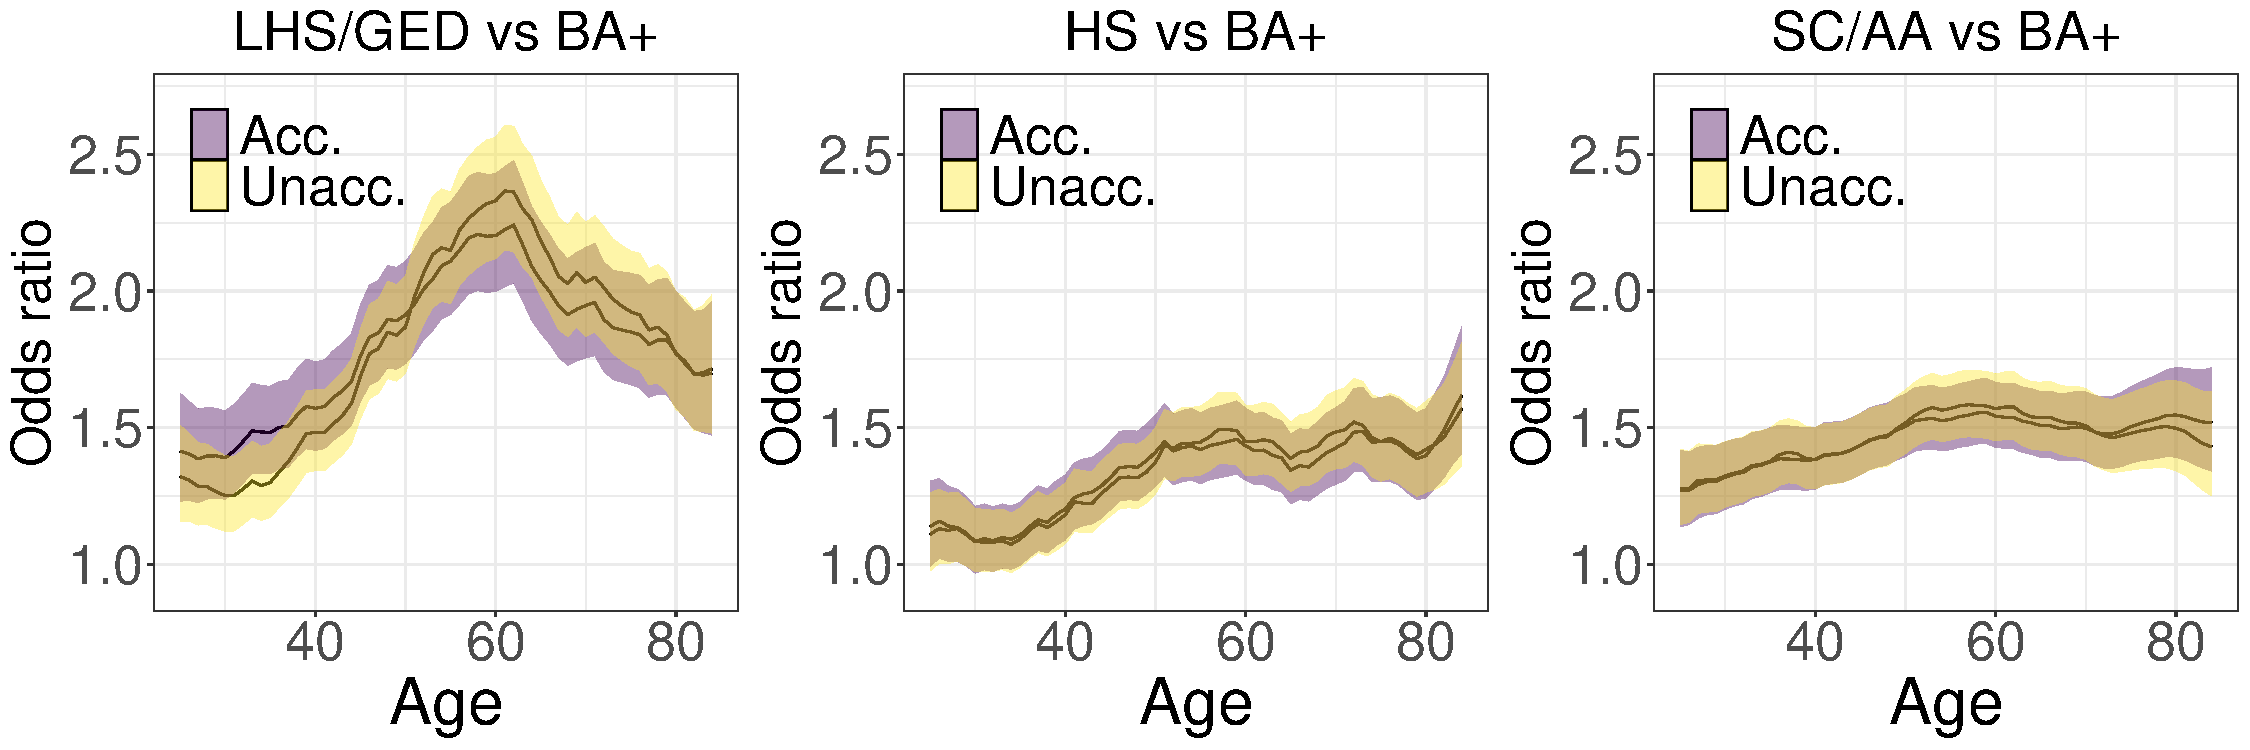
\includegraphics[width=\textwidth]{Figures/lincomb_hajek_f_age.pdf}
    \end{subfigure}
    \vskip\baselineskip\vspace{-0.3cm}
    \begin{subfigure}[t]{\textwidth}   
        \centering 
        \caption[]%
        {}    
        \label{figure:Application2:cohort_diff_f}
        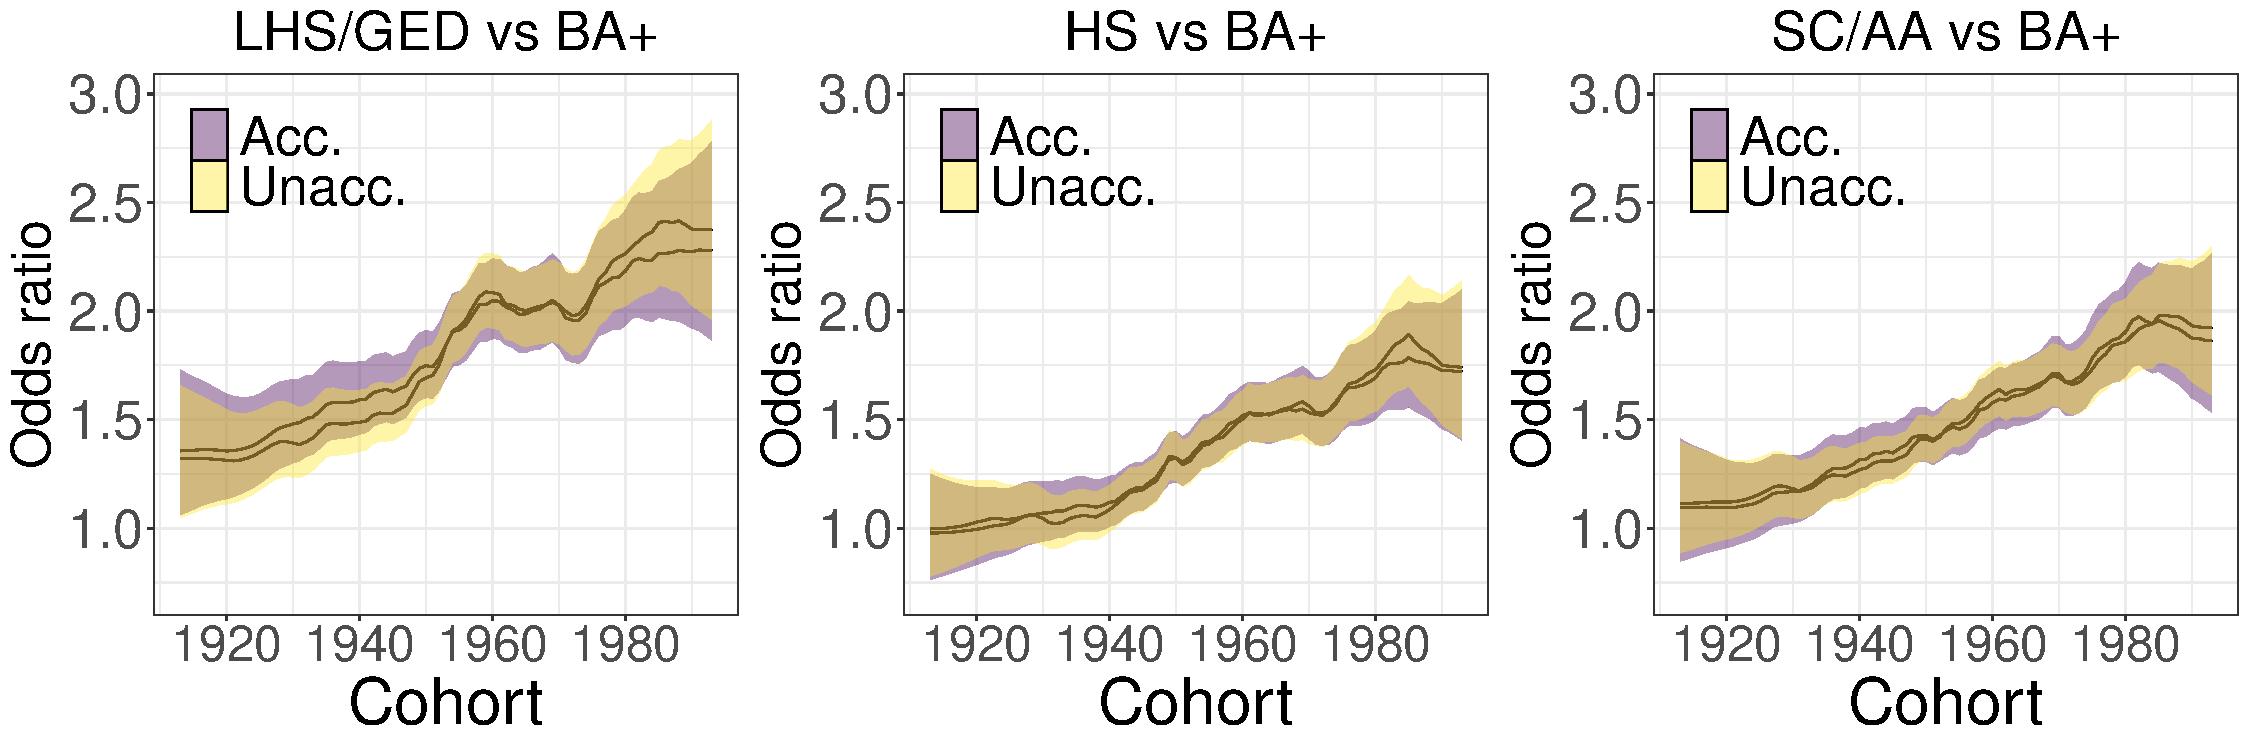
\includegraphics[width=\textwidth]{Figures/lincomb_hajek_f_cohort.pdf}
    \end{subfigure}
    \vspace{-0.2cm}
    \caption{Posterior median odds ratios together with $95\%$ credible intervals for less than high school (LHS), high school (HS), and some college/associate of arts degree (SC/AA) levels of attained education with respect to bachelor or higher education (BA+), over \textbf{(a)} age and \textbf{(b)} cohorts. The trends are shown for females using the aPc model accounting for the survey design, and are compared to the unaccounted estimates.}
    \label{figure:Application2:lincombs_f}
\end{figure}

%Best model males
\begin{figure}[h!]
    \centering
    \begin{subfigure}[b]{\textwidth}   
        \centering 
        \caption[]%
        {}    
        \label{figure:Application2:age_diff_m}
        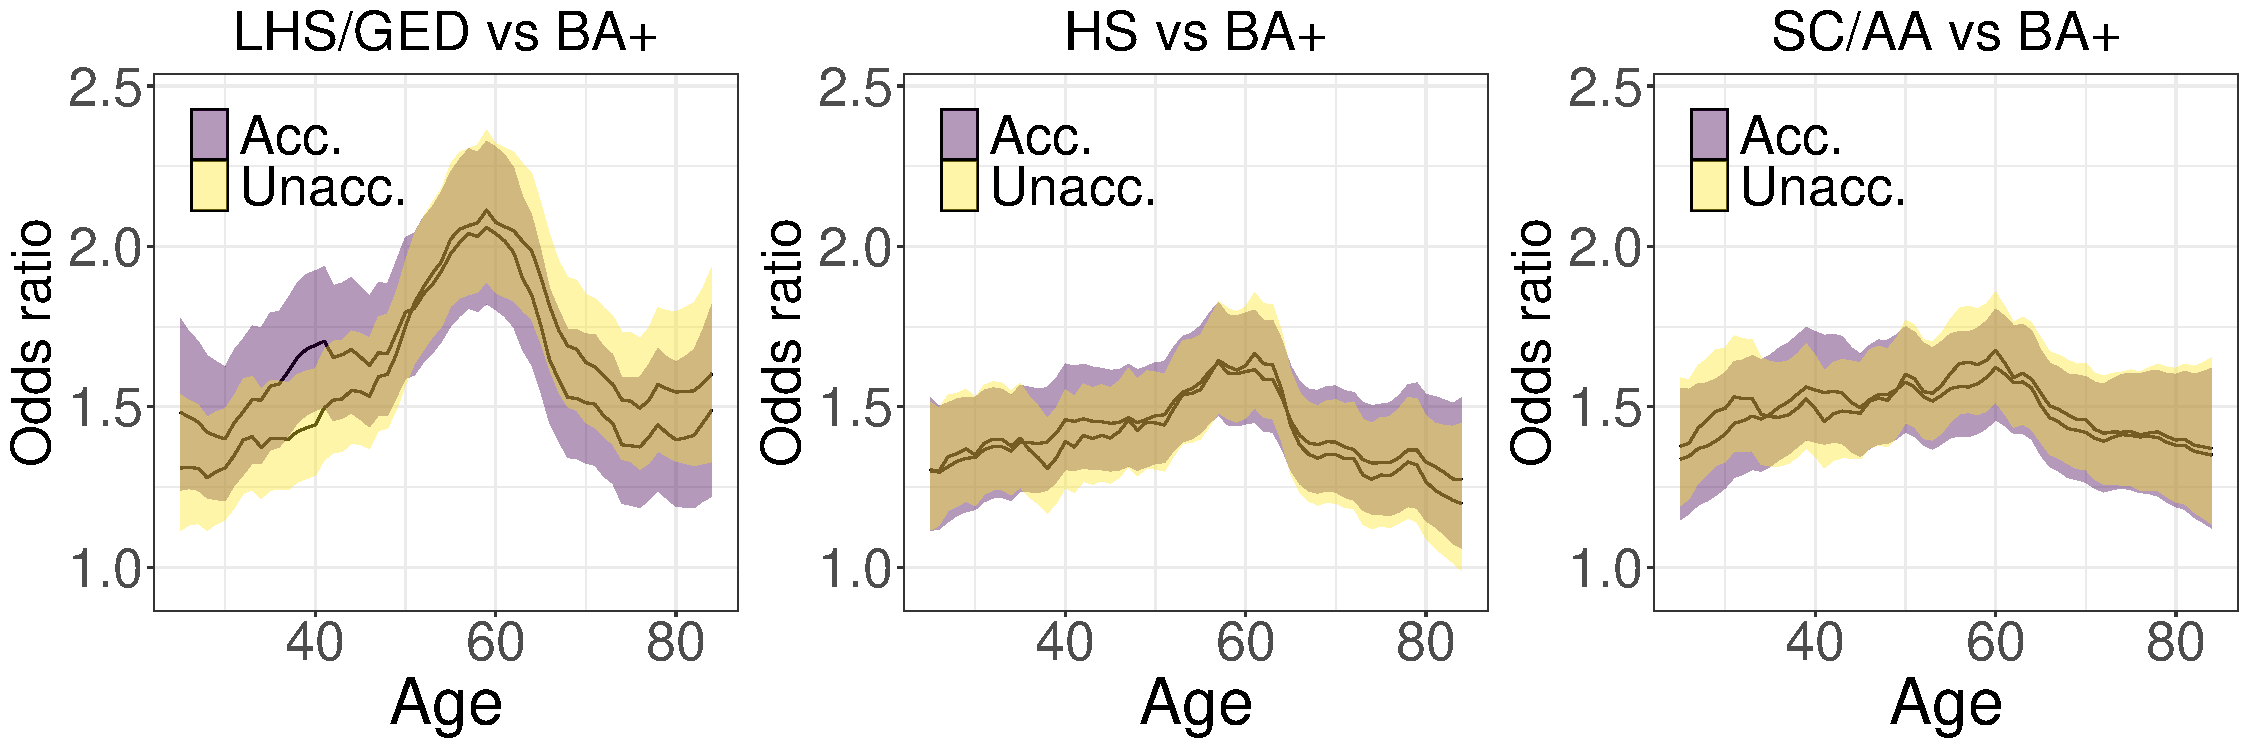
\includegraphics[width=\textwidth]{Figures/lincomb_hajek_m_age.pdf}
    \end{subfigure}
    \vskip\baselineskip\vspace{-0.3cm}
    \begin{subfigure}[b]{\textwidth}   
        \centering 
        \caption[]%
        {}    
        \label{figure:Application2:cohort_diff_m}
        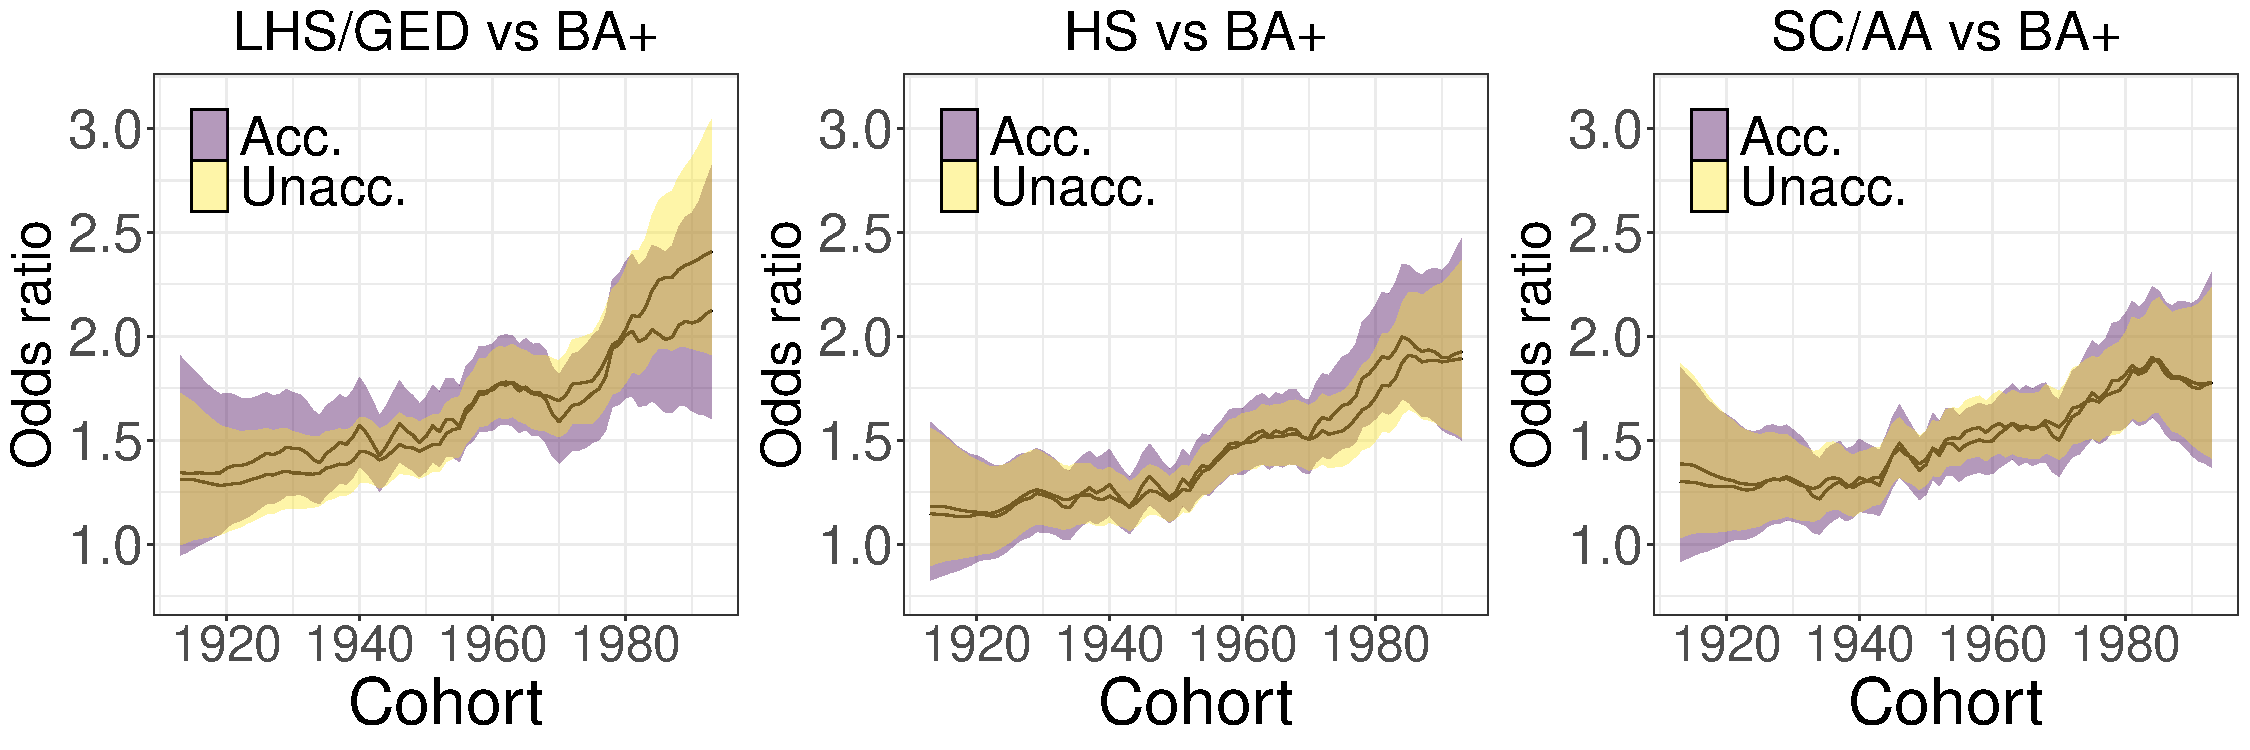
\includegraphics[width=\textwidth]{Figures/lincomb_hajek_m_cohort.pdf}
    \end{subfigure}
    \vspace{-0.2cm}
    \caption{Posterior median odds ratios together with $95\%$ credible intervals for less than high school (LHS), high school (HS), and some college/associate of arts degree (SC/AA) levels of attained education with respect to bachelor or higher education (BA+), over \textbf{(a)} age and \textbf{(b)} cohorts. The trends are shown for males using the aPc model accounting for the survey design, and are compared to the unaccounted estimates.}
    \label{figure:Application2:lincombs_m}
\end{figure}

%Over cohorts
\subsubsubsection*{Trends over cohorts}
\vspace{-0.2cm}
For the estimated odds ratios over cohorts in female and male data, seen in Figures \ref{figure:Application2:cohort_diff_f} and \ref{figure:Application2:cohort_diff_m}, the models accounting to the survey design appear to make similar estimates to the unaccounting models for all levels of attained education. Some different estimates are visible, though the differences are usually minor in the range between $0$ and $0.1$. That is, accounting for the complex sampling design does not change the overall pattern of the findings. There are, however, some differences, most notably for LHS/GED level of attained education compared to BA+ level in the most recent birth cohorts. Consequently, we again observe no overall change in the trends. In this region, notice that the credible intervals are very wide, meaning that there is higher uncertainty in the estimates. 

%Multiple models results
\subsubsubsection*{Trends in alternative models}
\vspace{-0.2cm}
The posterior medians of the odds ratio in the top four models chosen by model selection in Section \ref{section:application2:model_selection}, along with $95\%$ credible intervals are shown in Figure \ref{figure:Application2:lincombs_f_survey} for female data, and Figure \ref{figure:Application2:lincombs_m_survey} for male data. Figures \ref{figure:Application2:age_diff_f_survey} and \ref{figure:Application2:age_diff_m_survey} show the odds ratios over age in the aPc, apC, and aPC models. As observed in the same set of models when not accounting for the survey design, in Section \ref{section:application1:results}, the trends in odds ratio are very similar for the apC and aPC models, but they were significantly different from trends in the aPc model. Compared to the trends in the unaccounting models in Figures \ref{figure:Application1:age_diff_f} and \ref{figure:Application1:age_diff_m}, we observe more similarity between the trends in the models accounting for the survey design. In the odds ratios over period, in Figures \ref{figure:Application2:age_diff_f_survey} and \ref{figure:Application2:age_diff_m_survey}, we again have only one model to consider, namely the apC model. We observe trends that are either flat and then rise from 2005, or are slightly increasing overall. Interestingly, the trends using male data fluctuate less in the accounting models compared to the unaccounting models in Figures \ref{figure:Application1:age_diff_f} and \ref{figure:Application1:age_diff_m}. Over cohorts, in Figures \ref{figure:Application2:cohort_diff_f_survey} and \ref{figure:Application2:cohort_diff_m_survey}, we observe that the estimated trends in the aPc and APc models. The observations made for the cohort trends in the accounting models are similar to the trends of their unaccounting counterparts. In female data in particular, we again observe the steep drop for LHS/GED level of attained education in the APc model between the $1960$ and $1970$ cohorts. This drop is also visible when using the male data, though again to a lesser extent. Overall, when accounting for the survey design, the differences between models of different configurations of shared and stratum-specific effects are similar to those observed when not accounting for the design, albeit the differences are somewhat smaller in the design accounting models.

%Top3 models female
\begin{figure}[h!]
    \centering
    \begin{subfigure}[b]{\textwidth}   
        \centering 
        \caption[]%
        {}    
        \label{figure:Application2:age_diff_f_survey}
        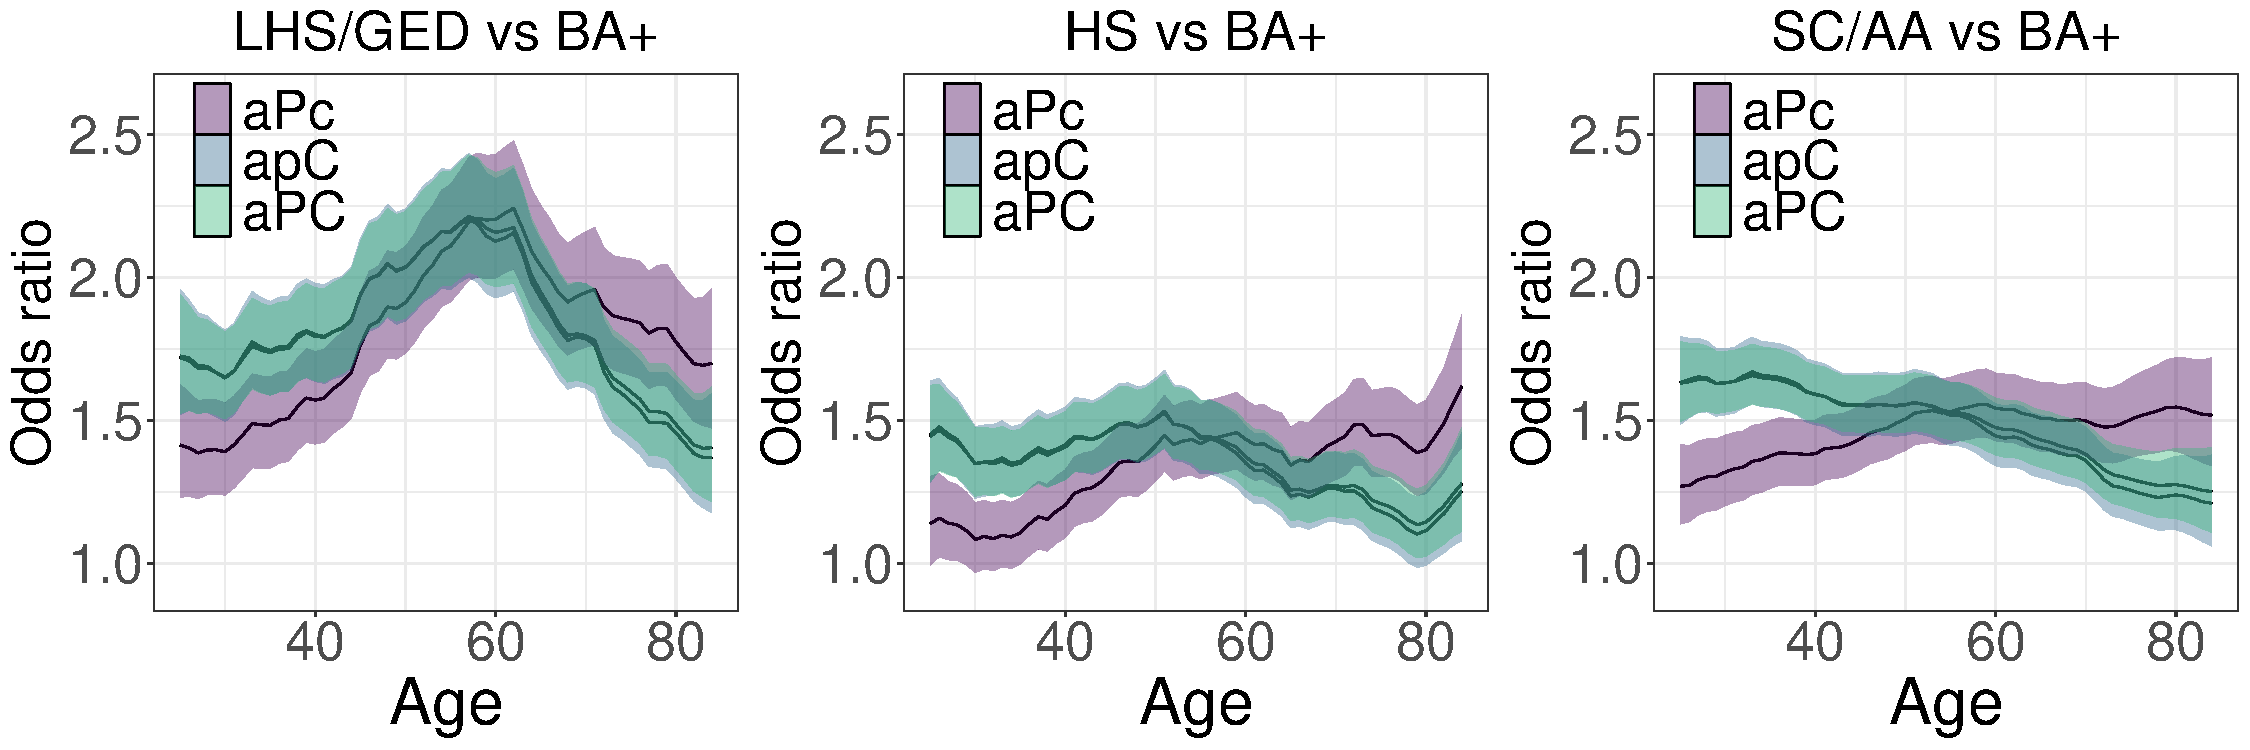
\includegraphics[width=\textwidth]{Figures/lincomb_age_f_survey.pdf}
    \end{subfigure}
    \vskip\baselineskip\vspace{-0.3cm}
    \begin{subfigure}[b]{\textwidth}   
        \centering 
        \caption[]%
        {}    
        \label{figure:Application2:period_diff_f_survey}
        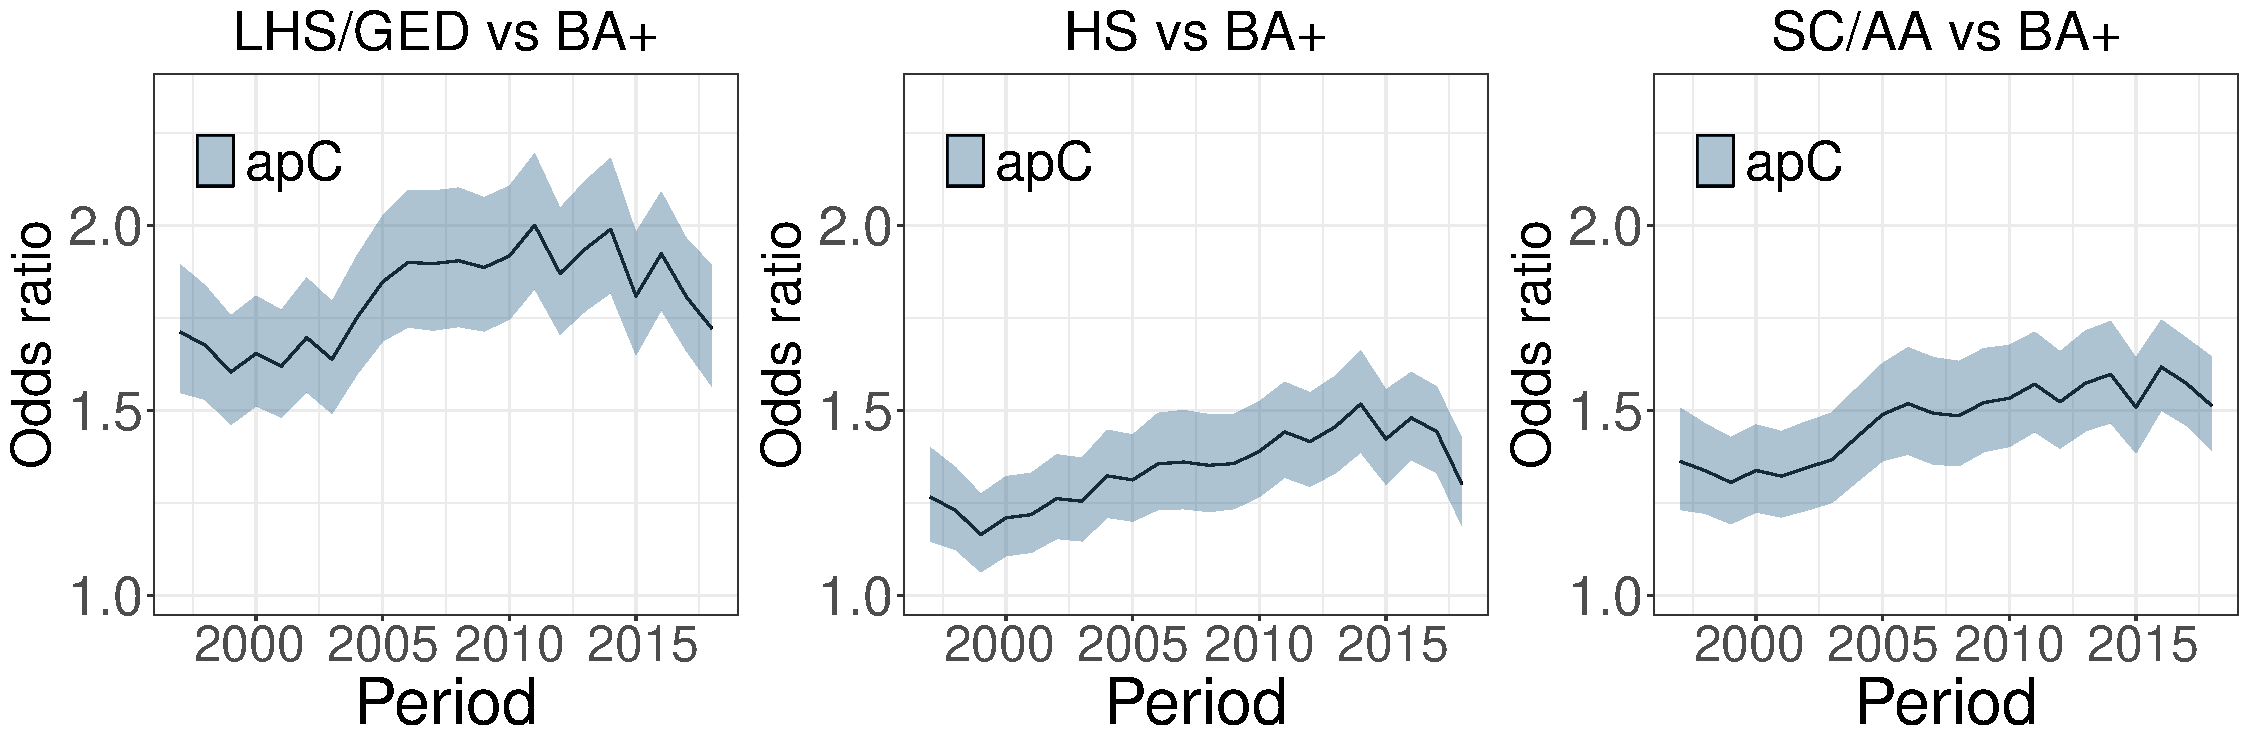
\includegraphics[width=\textwidth]{Figures/lincomb_period_f_survey.pdf}
    \end{subfigure}
    \vskip\baselineskip\vspace{-0.3cm}
    \begin{subfigure}[b]{\textwidth}   
        \centering 
        \caption[]%
        {}    
        \label{figure:Application2:cohort_diff_f_survey}
        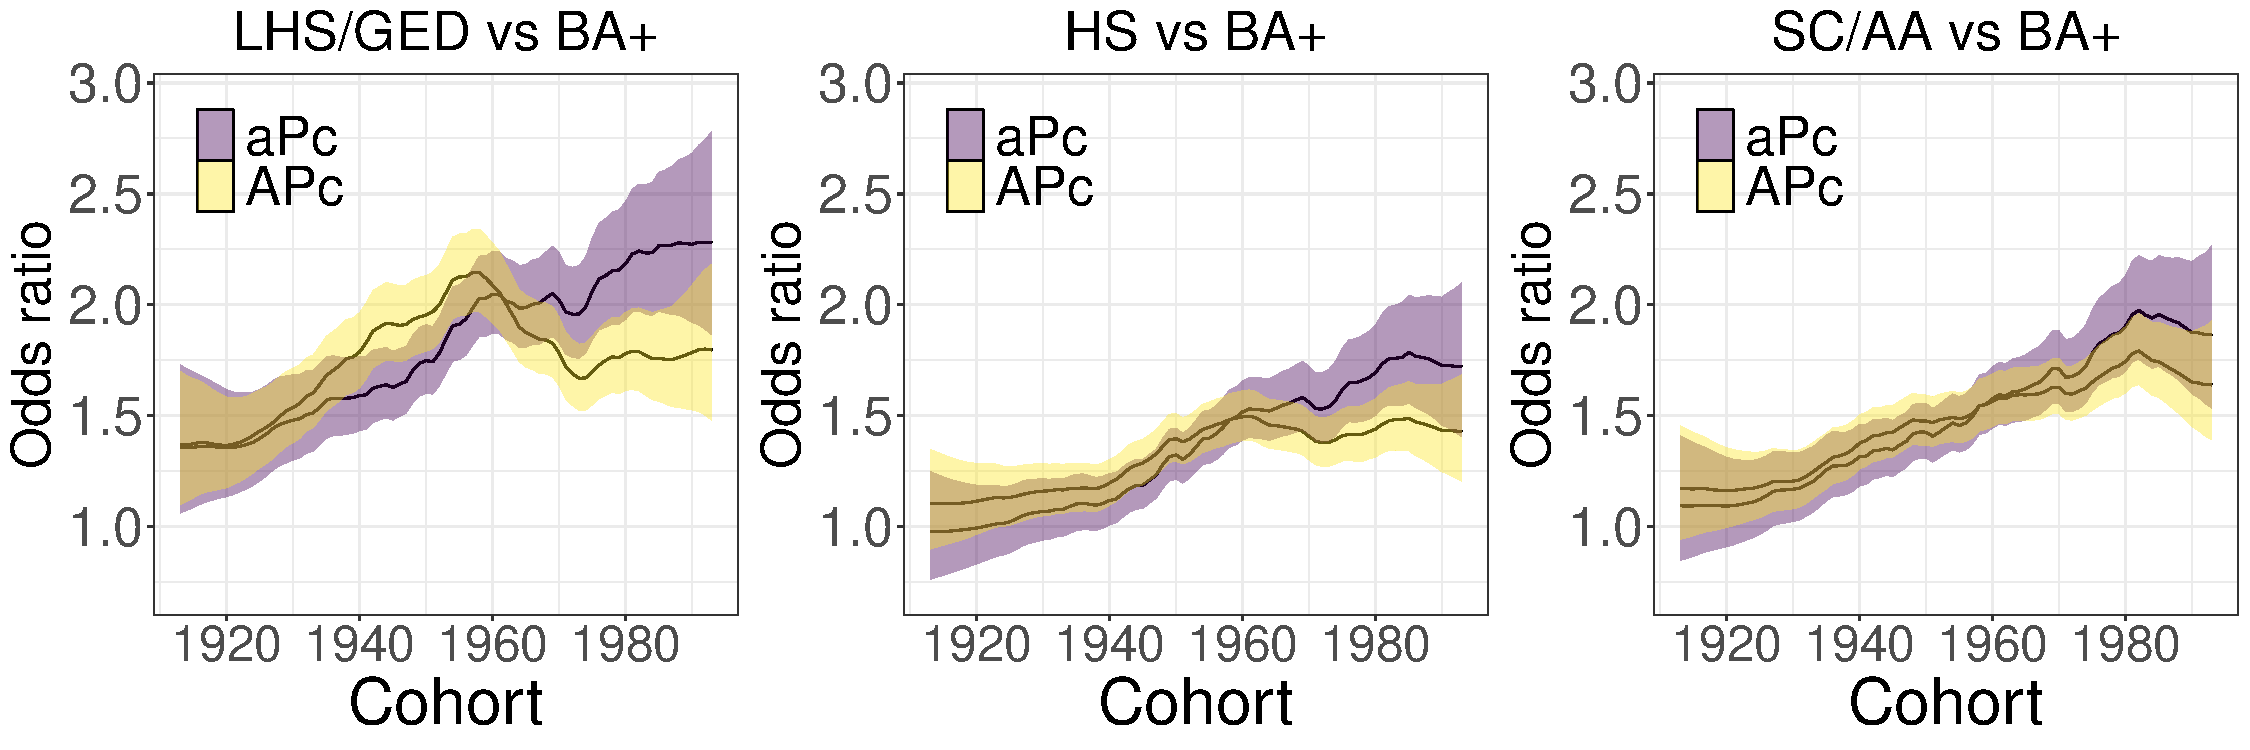
\includegraphics[width=\textwidth]{Figures/lincomb_cohort_f_survey.pdf}
    \end{subfigure}
    \vspace{-0.2cm}
    \caption{For females with less than high school (LHS), high school (HS), and some college/associate of arts degree (SC/AA) levels of attained education with respect to bachelor or higher education (BA+), the posterior median odds ratio in the top four models accounting for the survey design chosen by model selection over \textbf{(a)} age, \textbf{(b)} periods, and \textbf{(c)} cohorts, together with $95\%$ credible intervals.}
    \label{figure:Application2:lincombs_f_survey}
\end{figure}


%Top3 models male
\begin{figure}[h!]
    \centering
    \begin{subfigure}[b]{\textwidth}   
        \centering 
        \caption[]%
        {}    
        \label{figure:Application2:age_diff_m_survey}
        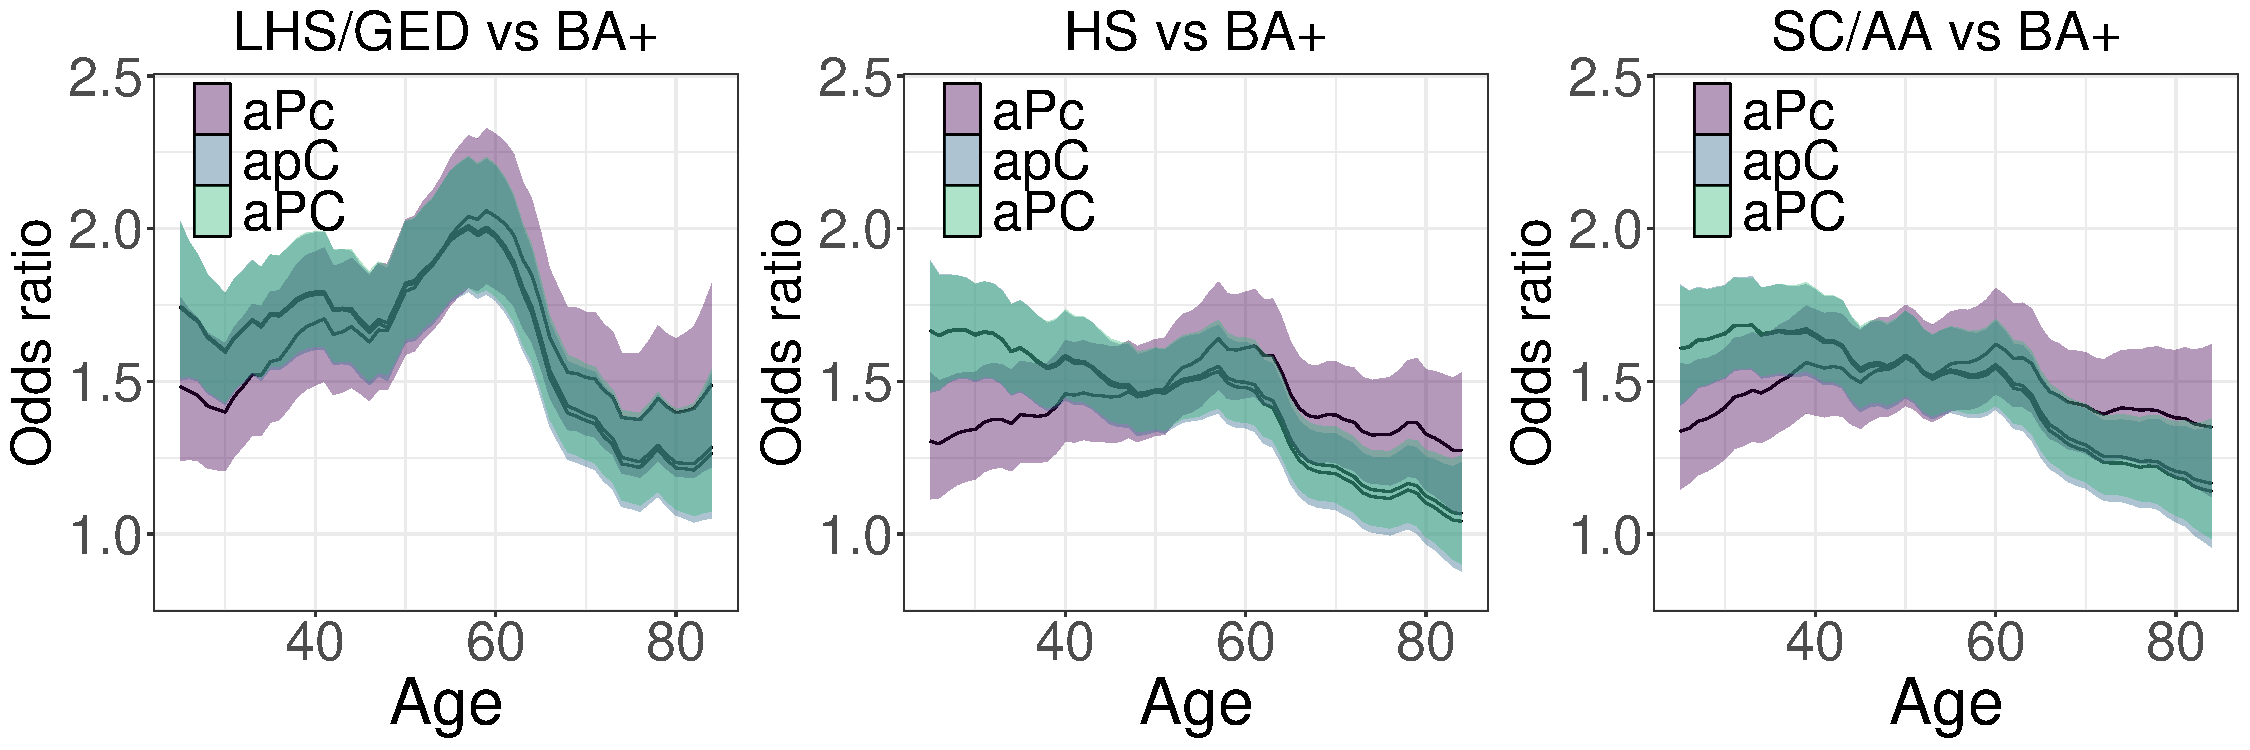
\includegraphics[width=\textwidth]{Figures/lincomb_age_m_survey.pdf}
    \end{subfigure}
    \vskip\baselineskip\vspace{-0.3cm}
    \begin{subfigure}[b]{\textwidth}   
        \centering 
        \caption[]%
        {}    
        \label{figure:Application2:period_diff_m_survey}
        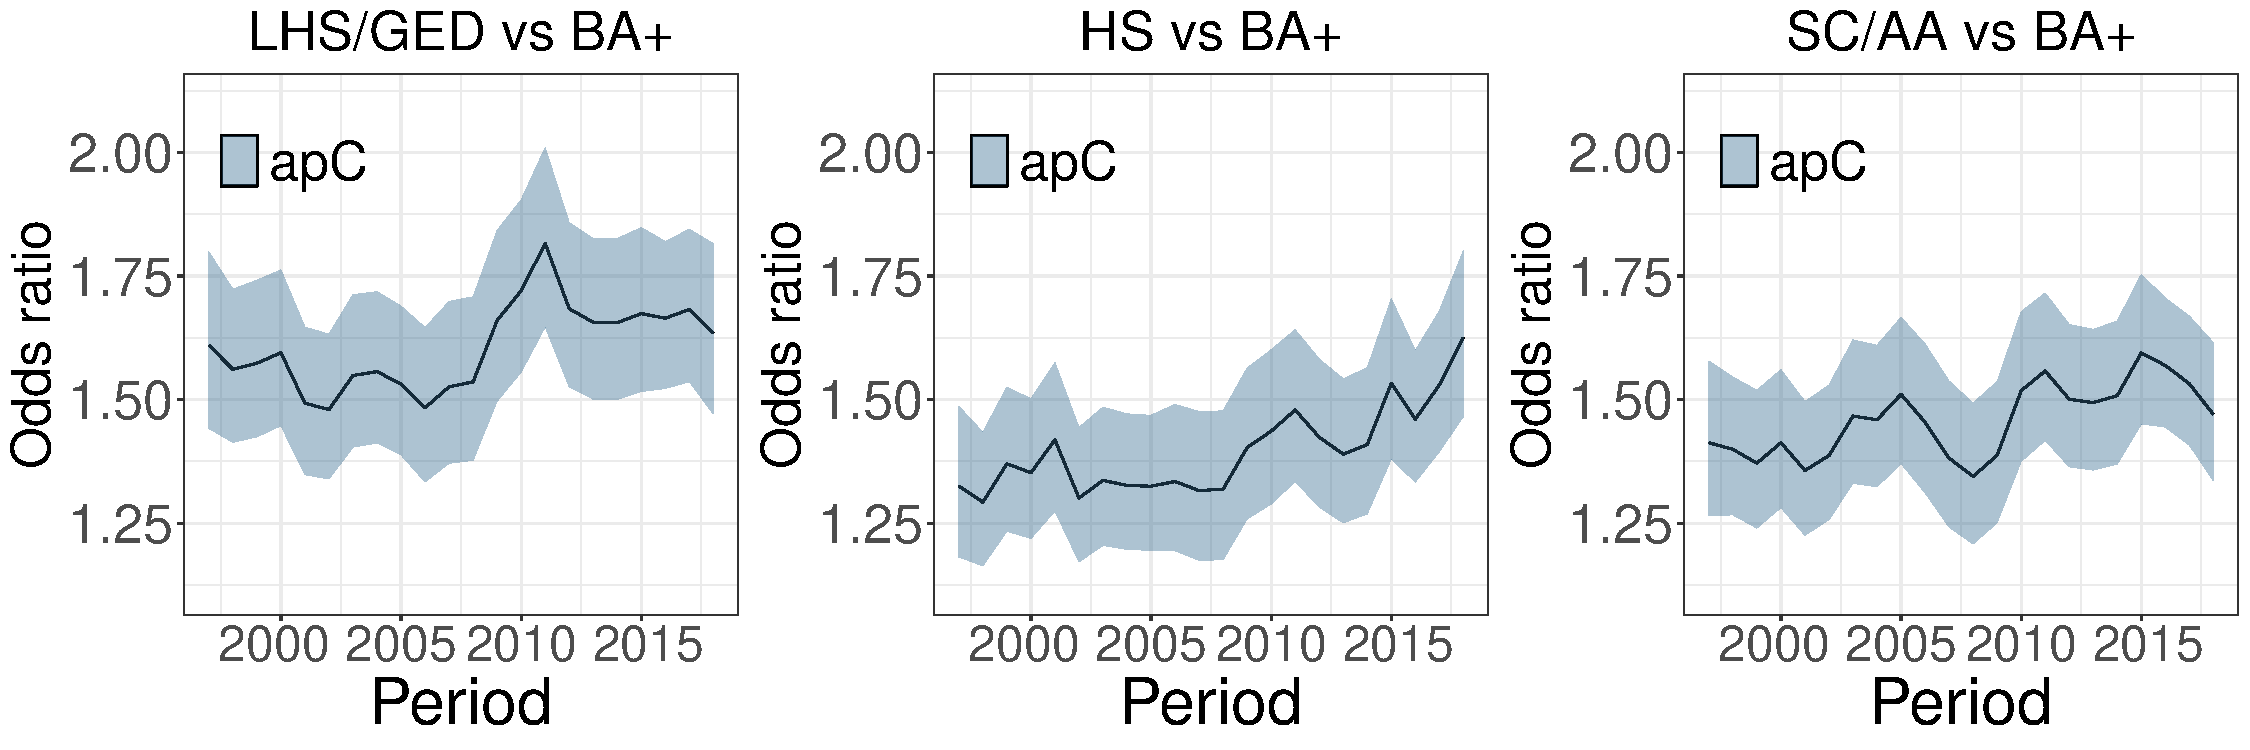
\includegraphics[width=\textwidth]{Figures/lincomb_period_m_survey.pdf}
    \end{subfigure}
    \vskip\baselineskip\vspace{-0.3cm}
    \begin{subfigure}[b]{\textwidth}   
        \centering 
        \caption[]%
        {}    
        \label{figure:Application2:cohort_diff_m_survey}
        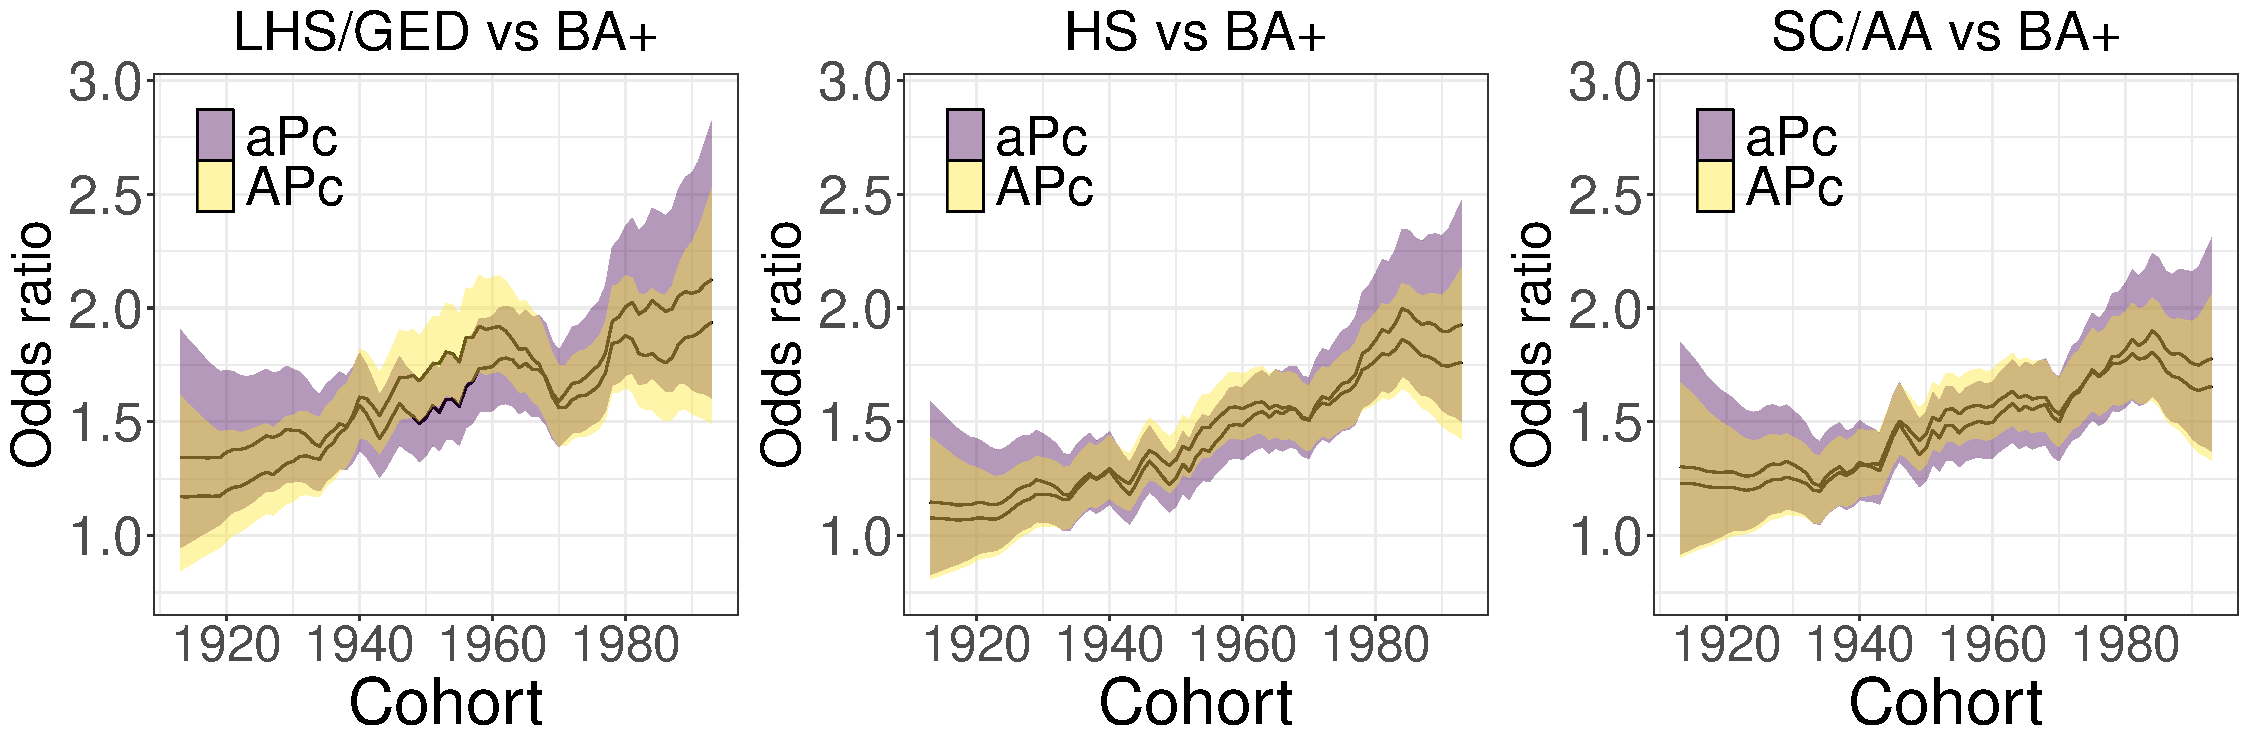
\includegraphics[width=\textwidth]{Figures/lincomb_cohort_m_survey.pdf}
    \end{subfigure}
    \vspace{-0.2cm}
    \caption{For males with less than high school (LHS), high school (HS), and some college/associate of arts degree (SC/AA) levels of attained education with respect to bachelor or higher education (BA+), the posterior median odds ratio in the top four models accounting for the survey design chosen by model selection over \textbf{(a)} age, \textbf{(b)} periods, and \textbf{(c)} cohorts, together with $95\%$ credible intervals.}
    \label{figure:Application2:lincombs_m_survey}
\end{figure}


\FloatBarrier
\subsection{Discussion}
\label{section:application2:discussion}
\subsubsubsection*{Summary}
\vspace{-0.2cm}
In this section, the survey design variables discussed in Section \ref{section:surveyData} were successfully incorporated in our Bayesian multivariate age-period-cohort model following the approach suggested by \cite{SurveyDesignMercer}. The survey design weights were included in the estimates using the Hájek estimator (Section \ref{section:application2:hajek}), while the PSU and STRATA design variables (Section \ref{section:surveyData}) were used to estimate the variance of the estimator. Computationally, the \texttt{survey} package was used to obtain the direct estimates with the corresponding variances. Model selection was carried out once more using logarithmic score, again selecting the aPc model with shared period effects, and stratum-specific age and cohort effects. Again, as discussed in Section \ref{section:APC-inference}, the estimated odds ratios are with respect to the highest level of education, BA+. 

%How compared to the regular results? Was the impact of survey designs great? Any further insights
\subsubsubsection*{Effects of accounting for the survey design}
\vspace{-0.2cm}
As we have seen from the estimated trends in the aPc model, the trends do not appear to change much when accounting for the survey design. Although the estimated odds ratios differ in certain regions, the overall shape, magnitudes, and interpretations of the trends remain largely the same in the accounting and unaccounting models. It is interesting to note that the width of the credible intervals appear to be roughly the same sizes in both the accounting and unaccounting models, meaning that aside from the different estimates caused by the survey weights, incorporating the survey design variables in the variance of the estimator did also not seem to affect the results much. Therefore, accounting for the survey design did not affect our conclusions to a great extent, but it does reassure us that our discussed points and interpretations on the unaccounting model in Section \ref{section:Application1:Dicussion} are still valid. While accounting for the survey design did not lead to different conclusions in this analysis, it cannot be said that this will be the case for all other analyses using APC models with different data. As we have demonstrated, accounting for the survey design weights in APC models is doable and does not require much extra effort. Therefore, it is recommended to incorporate these survey weights in future temporal analyses using APC models with survey data, to analyse the data properly.

%Variation in models
\subsubsubsection*{Trends in alternative models}
\vspace{-0.2cm}
Moreover, when accounting for the survey design, we saw that the estimated trends have become more similar between models with different combinations of shared and stratum-specific effects. Observing different trends when using different combinations of shared and stratum-specific effects is expected, since the underlying model assumptions are different. Over age, we still observe the inverse V-shaped trend for LHS/GED level of attained education, and over cohorts, we observe rising risk with more recent cohorts. An interesting twist lies in the trends over age for HS and SC/AA levels of attained education, where the alternative models without a stratum-specific cohort effect showed decreasing, rather than increasing trends. If we assume that the cohort effects are the same in all levels of attained education, we would then we observe that as participants with HS and SC/AA levels of attained education grow older, the risk of backpain compared to BA+ level is smaller. Thus, in these alternative models, the impact of education is considerably stronger in younger adults, and begins to even out to the levels observed for the BA+ level of attained education.

%Weirdness of GED still
\subsubsubsection*{Disparities in the LHS/GED educational group}
\vspace{-0.2cm}
In our comparison of the temporal trends between the accounting and unaccounting models, it was observed that the odds ratios differed the most for LHS/GED level of attained education. As has already been argued, the LHS/GED level of attained education stands out from the other levels of attained education by several measures. For this level, we have seen greater disparities in health and smaller sample sizes. Moreover, external socioeconomic factors for this level of education can be argued to have changed the most over the cohorts \citep{dowd2014life,montez2011trends,hendi2015trends}. Although accounting for the survey design did not provide much more insight into the trends of this level of attained education, the survey variables we incorporated still allow us to make better use of samples from subpopulations. Consequently, we will be continuing our analysis accounting for the survey design by considering only parts of the population.

\FloatBarrier
\subsection{Further investigation on a subpopulation}
\label{section:application2:extension}
Following our discussion of the observed trends in the aPc model when accounting for the survey design, in Section \ref{section:application2:discussion}, further investigation of the temporal trends is motivated, particularly for LHS/GED level of attained education. After consultation with the sociologist who provided us with the expert knowledge in Section \ref{section:application1:prior}, it was recommended to run the same analysis while accounting for the survey design using only white, U.S.-born participants. Other than education, critical driving factors of health include race/ethnicity and nativity. The composition of the LHS/GED educational group has changed dramatically over the years by several measures. One such measure is immigration, where many adult immigrants arrive with education corresponding to LHS/GED level. Consequently, for many of the years in their lives, they have been exposed to conditions and factors foreign to the U.S., in turn making the composition of the LHS/GED educational group more complex. Therefore, it would be interesting to see what happens to the temporal trends when we account for some effects of immigration. Since additional controls cannot be included at the moment, filtering the acquired NHIS survey data for only white, U.S-born participants may help mitigate potential confounding due to the changing composition of the educational groups. To this end, the same procedures to account for the survey design, as in Section \ref{section:application2:implementation}, are used on the subset of the data that includes only white, U.S.-born participants. Ideally, this would be compared against the complementary filtering, though this would create problems with data sparsity, since not every combination of age, period, cohort, and education would be represented in the data. Moreover, in this data, some triplets of age, period, and educational attainment level had no observations of back pain, and were remedied by fixing the observation to $0.01$ with an estimated variance of $1$, as before. This time, there were also some triplets in which all participants had back pain, and so this was remedied by fixing the observation to $0.99$, along with the estimated variance to $1$. The resulting temporal trends will be compared to those achieved using data on all participants, as presented in Section \ref{section:application2:results}. 

\subsubsection{Results}
\label{section:application2:extension:results}
\subsubsubsection*{Summary}
\vspace{-0.2cm}
By using the NHIS survey data on only white, U.S.-born participants, Figures \ref{figure:Application2:lincombs_f_filtered} and \ref{figure:Application2:lincombs_m_filtered} show the posterior median odds ratios in the aPc model when accounting for the survey design, along with $95\%$ credible intervals for females and males, respectively. The odds ratios are shown over age and cohorts in the respective subfigures, along with the corresponding estimates in the aPc model accounting for the survey design using survey data on all participants (as presented in Section \ref{section:application2:results}). For convenience, models using survey data on only white, U.S.-born participants are referred to as filtered models, while models using survey data on all participants is referred to as unfiltered models. As discussed in Section \ref{section:APC-inference}, all estimated odds ratios are with respect to the highest level of attained education, BA+. 

%Over age
\subsubsubsection*{Trends over age}
\vspace{-0.2cm}
Over age, in Figures \ref{figure:Application2:age_diff_f_filtered} and \ref{figure:Application2:age_diff_m_filtered}, we observe similar estimates of the odds ratios for HS and SC/AA levels of attained education. In females with these levels of attained education, the main differences between the filtered and unfiltered models are observed between age groups $25$ and $50$, with greater differences in males than females. Overall, the shape of the trends are similar, and the credible intervals overlap continuously, yielding no different interpretations. On the other hand, for LHS/GED level of attained education, noticeable differences in the estimated odds ratios are observed. In females, a nearly constant difference in odds ratio is observed between the filtered and unfiltered models, with the estimated median odds ratios being mostly outside the credible intervals of each other. The differences in odds ratio varies between $0.25$ and $0.4$, taking higher values in age groups younger than $60$. In females, this nearly constant difference is also observed, though also amplified to range between $0.25$ to $0.5$, again with larger differences in age groups younger than $60$. Consequently, we observe a much higher risk of back pain in the white, U.S-born population with LHS/GED level of attained education compared to the corresponding age groups with BA+ level of attained education. It is also worth noting that the credible intervals of odds ratios in the filtered models are much wider than their unfiltered counterpart only for LHS/GED level of attained education. 

%Over cohorts
\subsubsubsection*{Trends over cohorts}
\vspace{-0.2cm}
Over cohorts, as shown in Figures \ref{figure:Application2:cohort_diff_f_survey} and \ref{figure:Application2:cohort_diff_m_survey} for males and females, respectively, we again observe similarities between the filtered and unfiltered models for HS and SC/AA levels of attained education, and dissimilarities for LHS/GED level of attained education. For HS and SC/AA levels of attained education, the differences in odds ratios over cohorts compared to the differences over age is smaller, though there are some differences in the estimates of the most recent cohorts. Overall, these differences do not change the overall shape and interpretations of the trends. We observe major differences for LHS/GED level of attained education, though over cohorts these differences are expressed differently for each sex. For females in older cohorts, the differences in the estimated odds ratios are around $0.25$, increasing gradually to nearly $1.2$ by the most recent cohorts. At most, this yields an estimated odds ratio of $3.5$ for the most recent cohorts, and a minimum of $1.5$ for the oldest cohorts. In males, we observe similar estimates between the filtered and unfiltered models from the $1913$ to $1940$ birth cohorts, after which the odds ratios in the filtered models rapidly increases to $2.5$ by the $1960$ birth cohort, at which point the unfiltered model estimates odds ratios around $1.75$. Between the $1960$ and $1993$ birth cohorts, the estimates of the filtered model fluctuates a lot, though it decreases to estimates comparable to that of the unfiltered model by the $1993$ birth cohort. The credible intervals are again observed to be significantly wider in the filtered model than the unfiltered model for LHS/GED level of attained education. 

\begin{figure}[h!]
    \centering
    \begin{subfigure}[b]{\textwidth}   
        \centering 
        \caption[]%
        {}    
        \label{figure:Application2:age_diff_f_filtered}
        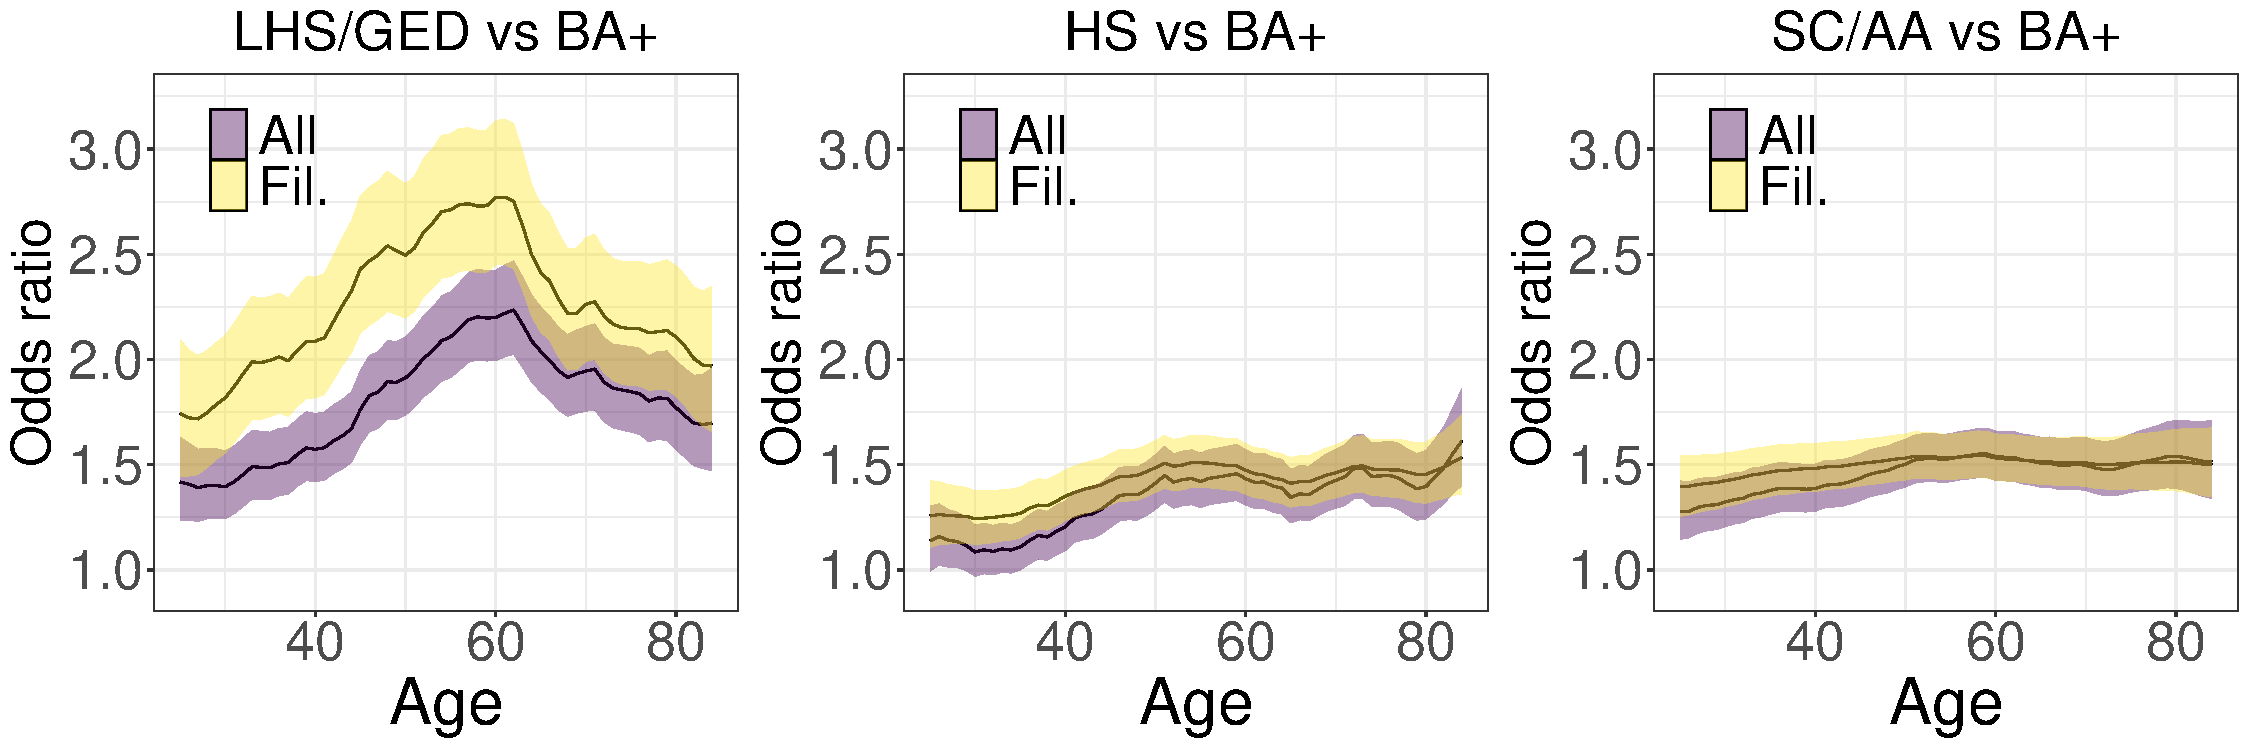
\includegraphics[width=\textwidth]{Figures/lincomb_survey_filtered_age_f.pdf}
    \end{subfigure}
    \vskip\baselineskip\vspace{-0.3cm}
    \begin{subfigure}[b]{\textwidth}   
        \centering 
        \caption[]%
        {}    
        \label{figure:Application2:cohort_diff_f_filtered}
        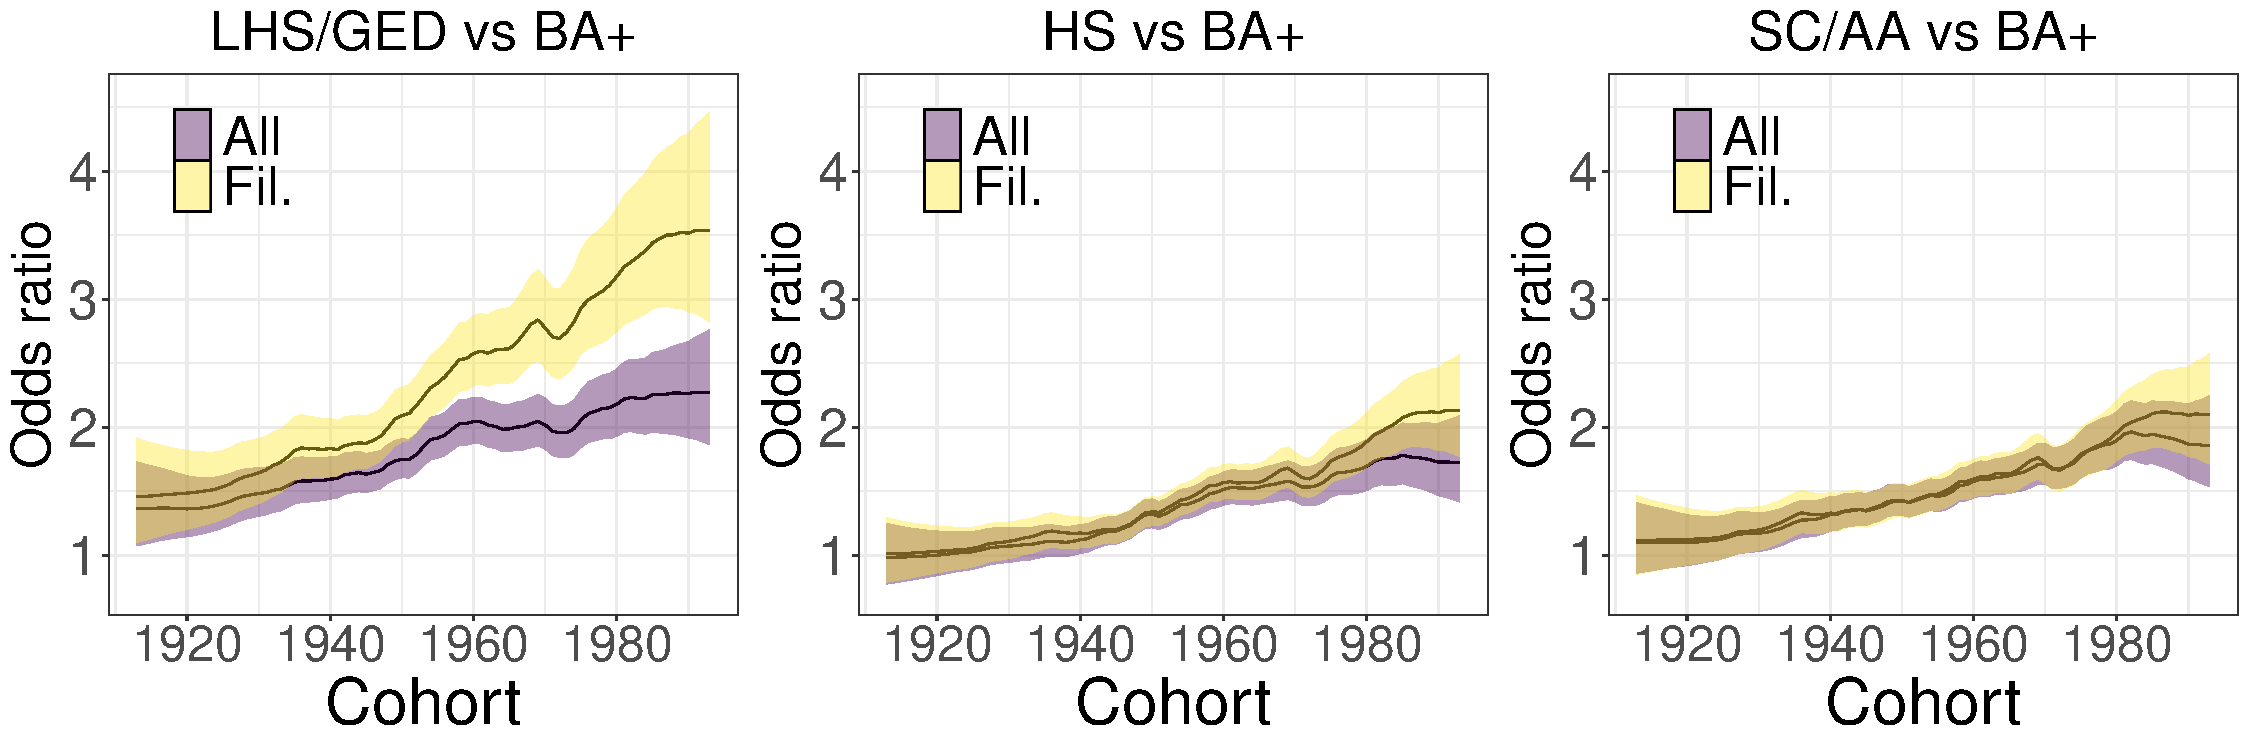
\includegraphics[width=\textwidth]{Figures/lincomb_survey_filtered_cohort_f.pdf}
    \end{subfigure}
    \vspace{-0.2cm}
    \caption{For less than high school (LHS), high school (HS), and some college/associate of arts degree (SC/AA) levels of attained education with respect to bachelor or higher education (BA+) level, the posterior median odds ratio over \textbf{(a)} age and \textbf{(b)} cohorts, in the aPc model accounting for the survey design along with $95\%$ credible intervals. The trends are shown using all female data (All) and using data on only white, U.S.-born females (Fil.).}
    \label{figure:Application2:lincombs_f_filtered}
\end{figure}

\begin{figure}[h!]
    \centering
    \begin{subfigure}[b]{\textwidth}   
        \centering 
        \caption[]%
        {}    
        \label{figure:Application2:age_diff_m_filtered}
        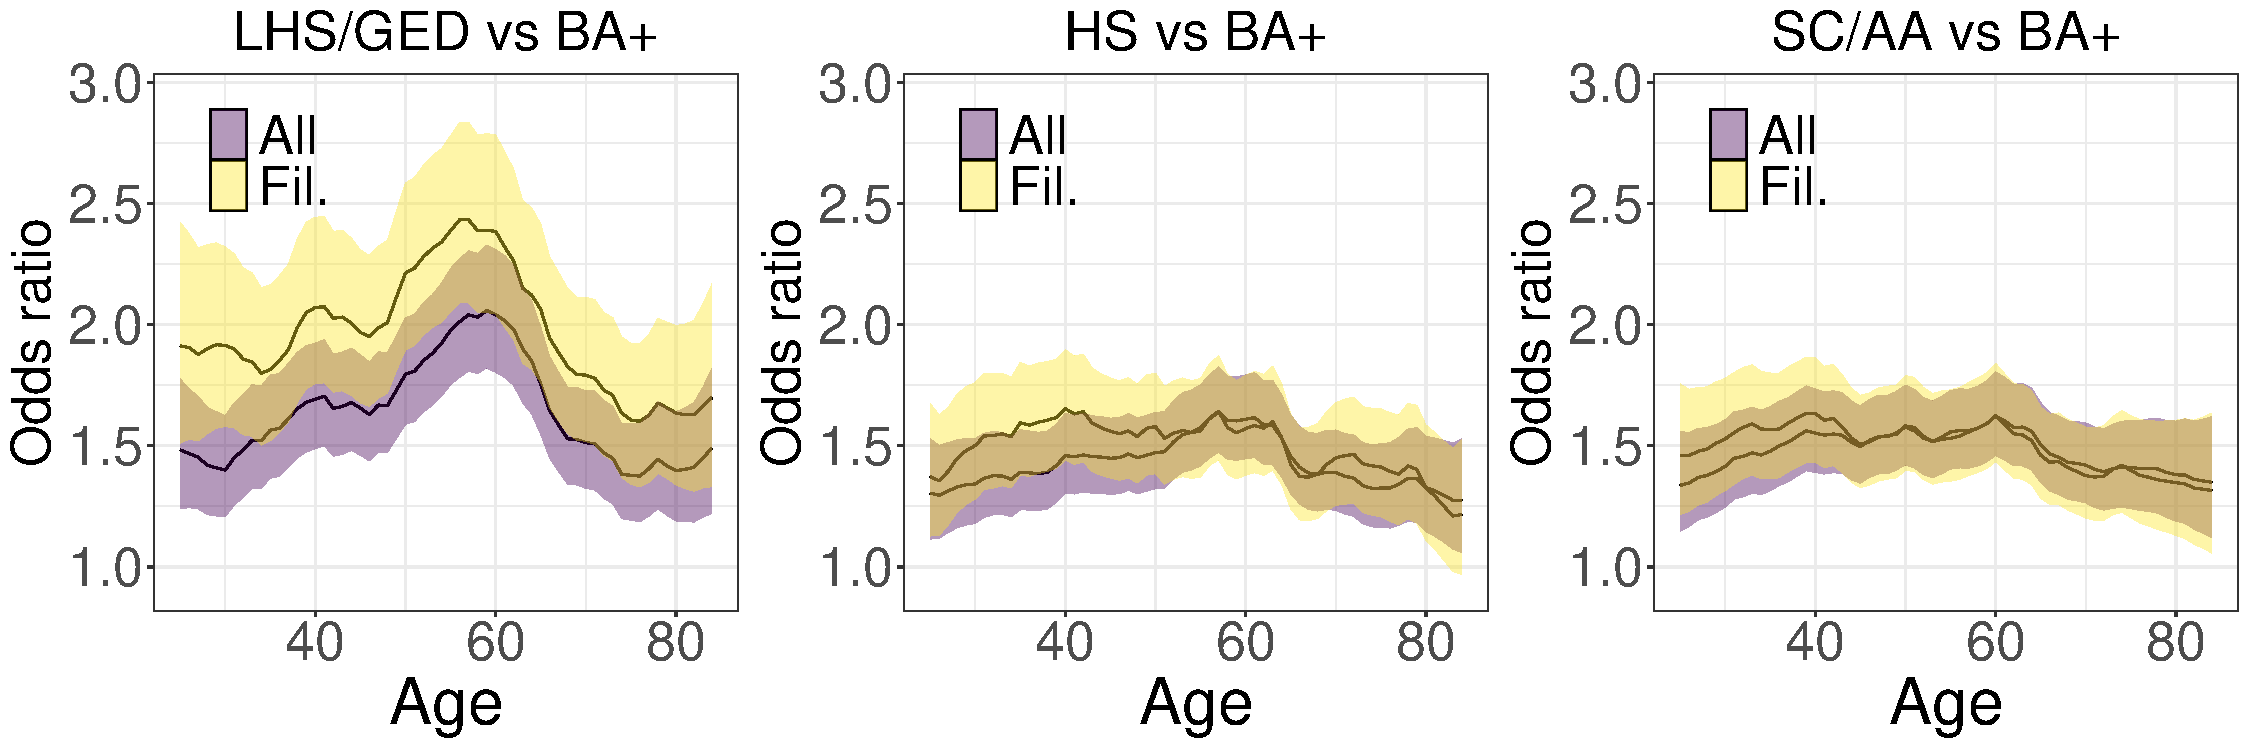
\includegraphics[width=\textwidth]{Figures/lincomb_survey_filtered_age_m.pdf}
    \end{subfigure}
    \vskip\baselineskip\vspace{-0.3cm}
    \begin{subfigure}[b]{\textwidth}   
        \centering 
        \caption[]%
        {}    
        \label{figure:Application2:cohort_diff_m_filtered}
        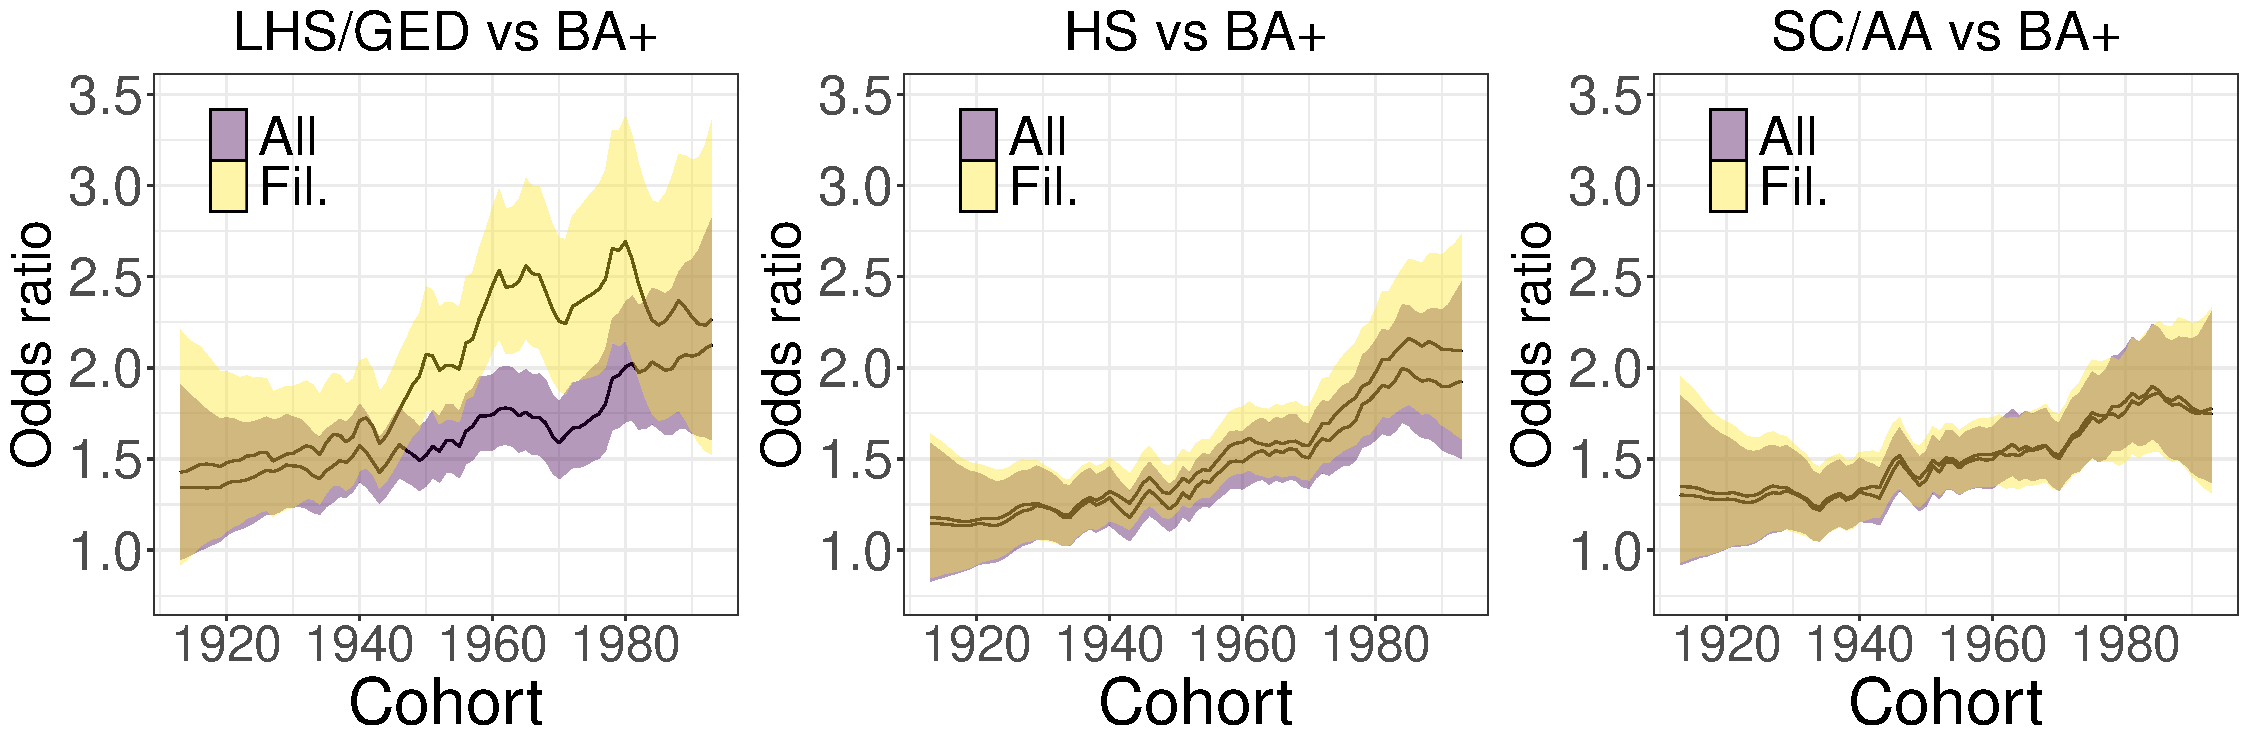
\includegraphics[width=\textwidth]{Figures/lincomb_survey_filtered_cohort_m.pdf}
    \end{subfigure}
    \vspace{-0.2cm}
    \caption{For less than high school (LHS), high school (HS), and some college/associate of arts degree (SC/AA) levels of attained education with respect to bachelor or higher education (BA+) level, the posterior median odds ratio over \textbf{(a)} age and \textbf{(b)} cohorts, in the aPc model accounting for the survey design along with $95\%$ credible intervals. The trends are shown using all male data (All) and using data on only white, U.S.-born males (Fil.).}
    \label{figure:Application2:lincombs_m_filtered}
\end{figure}

\subsubsubsection*{Additional smoothing}
\vspace{-0.2cm}
Using the filtered data, Figures \ref{figure:Application1:rw2_f_fil} and \ref{figure:Application1:rw2_m_fil} show the odds ratio trends over age and cohorts in the aPc model using RW1 and RW2 priors on the components of the latent field, for females and males respectively. As expected, the model using RW2 priors on the components of the latent field shows smoother temporal trends. The general shape of the trends are the same as when using RW1 priors, meaning that the introduction of more smoothing on the latent field did not drastically change the trends. 

\FloatBarrier
\subsubsection{Discussion}
\label{section:application2:extension:discussion}
In this short additional investigation, we attempted to eliminate the effects of some of the external factors that may have been present in particular for the LHS/GED educational group, by selecting only white, U.S.-born individuals for our analysis. Relying on the survey design adjustments, we saw that despite selecting only a subset of the total participants, we achieved estimates with similar uncertainty as in the model that uses all participants with HS and SC/AA levels of attained education. On the other hand, for LHS/GED level of attained education, large differences were observed between the models, with the filtered model displaying much larger credible intervals, resulting in more uncertainty in the estimated odds ratios. Despite the larger credible intervals, we identify regions in which the credible intervals of the models do not overlap, indicating that the differences are quite noticeable. 

In interpreting these results, it is important to keep in mind that in the filtered and unfiltered models, the educational group we compare against, BA+, is also affected by the filtering. That is, in the filtered model, we compared white, U.S.-born participants with LHS/GED level of attained education, to the white, U.S.-born participants with BA+ level of attained education. Though we expect the effects of immigration to be expressed the most for LHS/GED level of attained education, it may also affect the other levels of education as well. Should the white, U.S.-born only subset of the BA+ educational group be comparable to the BA+ educational group as a whole, one may then argue that our results show increased disparities in risk of back pain. If the white, U.S.-born subset of the BA+ educational group is different from the whole, then the observed differences could be due to the better health of this subpopulation. However, since we observed very similar trends for HS and SC/AA levels of attained education compared to BA+, it appears that the LHS/GED level of education is the odd one out once more. Consequently, our results indicate larger educational differences in the white, U.S.-born participants, though the aid of sociologists are again needed to further discuss potential causes of the observed differences. 














